\documentclass[12pt, a4paper]{report}
\usepackage{graphicx, array, amsthm, amssymb, amsmath, float, xcolor, thmtools, thmbox, geometry}
\usepackage[english]{babel}
\geometry{a4paper, left=2cm, right=2cm, top=2.5cm, bottom=2.5cm}
\newcounter{useCase}
\stepcounter{useCase}
\newcommand{\usecase}[9]{
    \def\arraystretch{1.5} 
    \subsubsection*{Use case [U#2]: #3}
    \vspace*{0.2cm}
    \begin{center}
        \begin{tabular}{|l|p{12cm}|}
            \hline
            \textbf{Actor(s)} & #4 \\
            \hline
            \textbf{Entry Condition} & #5 \\
            \hline
            \textbf{Event Flow} & #6 \\
            \hline
            \textbf{Exit Condition} & #7 \\
            \hline
            \textbf{Exceptions} & #8 \\
            \hline
            \textbf{Notes} & #9 \\
            \hline
        \end{tabular}
    \end{center}
    #1
}

\title{Requirement Analysis and Specification Document}
\author{Christian Rossi \\ Kirolos Sharoubim}
\date{Academic Year 2023-2024}

\begin{document}

\maketitle

\newpage

\tableofcontents

\newpage

\chapter{Introduction}
    \section{Purpose}
    CodeKataBattle is a platform employed by educators to challenge students on code Katas, problems meant to be tackled using a programming language selected by 
    the organizers of the challenge.
    
    Specifically, educators have the capability to establish a code Kata within a particular tournament by defining the following parameters: the problem to be solved 
    (with some test cases), the minimum and maximum number of students per group, and the deadlines for code Kata registration and solution submission.
    
    After the creation of the tournament, students can form groups and start their work on the solution, employing a test-first approach. When the ultimate deadline 
    approaches, the system autonomously calculates the final rankings and unveils the winners.

    \subsection{Goals}
    The goals, wich are the objectives to accomplish are the following
    \begin{enumerate}
        \item The system should allow students to join tournaments.
        \item The system should allow students to join battles as groups or individually in a specific tournament.
        \item The system should allow educators to manage a tournament.
        \item The system should allow educators to manage a battle in a specific tournament.
        \item The system should allow students and educators to see battles and tournaments rankings.
    \end{enumerate}


    \section{Scope}
    To ensure the proper development of this application, it is crucial to examine all imaginable phenomena linked to the system.
    
    These phenomena can be categorized into three distinct categories: world phenomena (occurring in the external environment beyond the machine's control), machine 
    phenomena (taking place within the machine and beyond the influence of the external world), and shared phenomena (interactions and events involving both the system
    and the external world).

    Regarding CodeKataBattle, we encounter the following external phenomena: 
    \begin{enumerate}
        \item The educator generates a code Kata problem description.
        \item The educator formulates a series of test cases for the code Kata problem.
        \item The students develop a program to solve the code Kata.
        \item The educator assigns a personal score based on code quality.
    \end{enumerate}
    Additionally, the following internal phenomena arise within the system: 
    \begin{enumerate}
        \item The system creates a GitHub repository.
        \item The system establishes an automated workflow through GitHub Actions to notify CKB about new commits.
        \item The system analyzes the repositories at every commit.
        \item The system conducts automated evaluation and updates the score according to the following criteria:
            \begin{enumerate}
                \item Number of passed test cases.
                \item Timeliness between the start of the challenge and the last commit on the main branch.
                \item Static code analysis for security, reliability, and maintainability.
            \end{enumerate}
    \end{enumerate}    
    Lastly, the following shared interactions and events emerge:
    \begin{enumerate}
        \item The educator initiates a battle on the platform, including the following steps:
            \begin{enumerate}
                \item Uploading the code Kata.
                \item Specifying the minimum and maximum number of students per group.
                \item Setting a registration deadline.
                \item Setting a final submission deadline.
                \item Configuring additional scoring parameters.
            \end{enumerate}
        \item Students submit their implementations to the platform via GitHub commits.
        \item The educator creates a tournament.
        \item The educator grants permissions to other educators to create code Kata within a specific tournament.
        \item Students subscribe to specific tournaments.
        \item The student joins an already existing group.
        \item The student forms a new group and extends invitations to other students.
        \item The educator concludes the tournament, and the system notifies the students.
    \end{enumerate}

    
    \section{Definitions, acronyms and abbreviations}
    \subsection{Definitions}
    \textbf{Code Kata}: adaptation of the concept of karate katas, where you repetitively refine a form, to the realm of software development, 
        fostering iterative practice and improvement. 
    \\
    \textbf{Test-first approach}:  software development process relies on the transformation of software requirements into test cases before 
        the software is completely developed, and it involves monitoring the entire software development by iteratively testing the software 
        against all these test cases.
    \subsection{Acronyms}
    \textbf{CKB}: CodeKataBattle 
    \\
    \textbf{CK}: Code Kata
    \subsection{Abbreviations}
    

    \section{Revision history}
    \textbf{Version 1.0} - Release - date TBD


    \section{Reference documents}
    \textbf{Document 1} - Presentation about RASD structure
    \\
    \textbf{Website 1} - http://codekata.com
    \\
    \textbf{Website 2} - https://en.wikipedia.org


    \section{Document structure}
    This document contains the following elements: 
    \begin{enumerate}
        \item \textbf{Introduction}: this section offers a general overview of CodeKataBattle and its objectives.
        \item \textbf{Overall description}: this section provides comprehensive information about the system, including interfaces, constraints, domain assumptions, software dependencies, and user characteristics.
        \item \textbf{Specific requirements}: this section outlines the system's functionalities through scenarios and use case diagrams.
        \item \textbf{Formal analysis with alloy}: this section contains the Alloy employed to verify the platform's correctness.
        \item \textbf{Effort spent}: this section details the amount of time (in hours) contributed by each group member.
        \item \textbf{References}: this section lists the tools used in the document's development.
    \end{enumerate}

\chapter{Overall description}
    \section{Product perspective}
    \subsection{Scenarios}
    \begin{enumerate}
        \item \textit{New user joins the platform}\\
            Maria is a Computer science student. Maria wrote a simple program in Java for a school project a month ago, and realised she really enjoys it. 
            Thus, she is looking for a chance to improve her Java skills as she didn't feel always confident about all the code she wrote.
            While searching online, Maria finds the CodeKataBattle platform and, as some challenges were exactly what she was looking for, she signs up: she inserts her email and a password and procedes as a student.
            A verification email is sent and, once the mail is verified by clicking the link in the verification email, she can start browsing the available tournaments looking for an interesting battle.
        
        \item \textit{Educator creates a new tournament} \\
            Anne is a professor in an engineering university.
            She teaches a course about optimization of problems' solution.
            One day she hears from a colleague of her, who's a computer science professor, about a platform called CodeKataBattle, which allows students to compete solving programming problems.
            Anne enjoys writing some python scripts to solve simple problems of everyday life and, while writing the scripts, she noticed that they required a deeper understanding of the solution.
            Since she knows that her students enjoy programming, as herself, Anne decides to create a tournament on CodeKataBattle, with the objective to make her students implement algorithms for the methods of problem-solving taught in the course.
            At first, she was not sure that she could make something so complex but the fact that the platform could assign automatically the ranking needing only some test cases and that multiple programming languages were supported made Anne change her mind.
            Thus, Anne creates a new tournament by setting a name and a deadline. All the students subscribed to CodeKataBattle are notified by the platform and can now subscribe.
        \item \textit{Educator adds a CK to a specific tournament} \\
            Jamie is a high school programming teacher; he is a Python and JavaScript expert but also knows Java.
            Jamie has been using CodeKataBattle for a while, since it helps his students to challenge themselves and provides an interactive programming exercise.\\
            Every year a CodeKataBattle tournament is held by the professor and based on the final ranking the students get some extra points in the exam grade.\\ 
            For this year, Jamie just found out an interesting problem that can be solved in various ways, each of them exploiting different proprieties of python.
            Thus, he decides to upload the problem in the tournament, not allowing students to join in groups since he wants to test each student individually.\\
            Therefore, Jamie creates five test cases, sets the deadline date and proceeds to upload the CodeKata, the registration deadline, the submission deadline and an additional scoring criteria on cleanliness of the code.
        \item \textit{Student joins a group for a specific CK in a tournament}\\
            Donald is a car wash employee, even if things are going great his dream was to become a web developer.
            Donald already learned a lot JavaScript and is always in search of new challenges.
            Donald knows that in programming environment team working is a must.
            Since he always studied and exercised alone on CodeKataBattle, he now wants to practice some team work.
            So Donald opens CodeKataBattle and looks for some tournaments were battles in numerous groups are allowed.
            Once he found some battles about topics he's interested in, where groups are allowed, he creates a group and waits for other students to join.
        \item \textit{Student does a commit} \\
            Charlotte and Matt are working on the solution of a battle in their teacher tournament.
            They thought every test was passed, but then, they realised there might be a particular case in which their algorithm fails.
            Thus, they fix the bug and, once they think the algorithm is done, the changes are committed and pushed.
            At this point the CodeKataBattle platform performs the tests, the static analysis and the time ranking, giving the two students a new higher rank, confirming that there was a bug in their code.
        \item \textit{Educator closes the tournament} \\
            Jeremiah is an Educator on CodeKataBattle, each month he creates a tournament about a simple problem, with a couple battles,
            one is usually a simple exercise, while the second is a more complex variation of the first one.
            As the month is coming to its end Jeremiah opens CodeKataBattle platform and checks how the participants are doing and decides to close the tournament.
            The platform then proceeds to assign the final ranking and score of each student subscribed to the tournament and makes them available for everyone to consult. 
    \end{enumerate}

    \subsection{Domain class diagrams}
    The domain class diagram for CodeKataBattle is presented below, covering all the elements within the system's operational environment and illustrating their interactions.
    \begin{figure}[H]
        \centering
        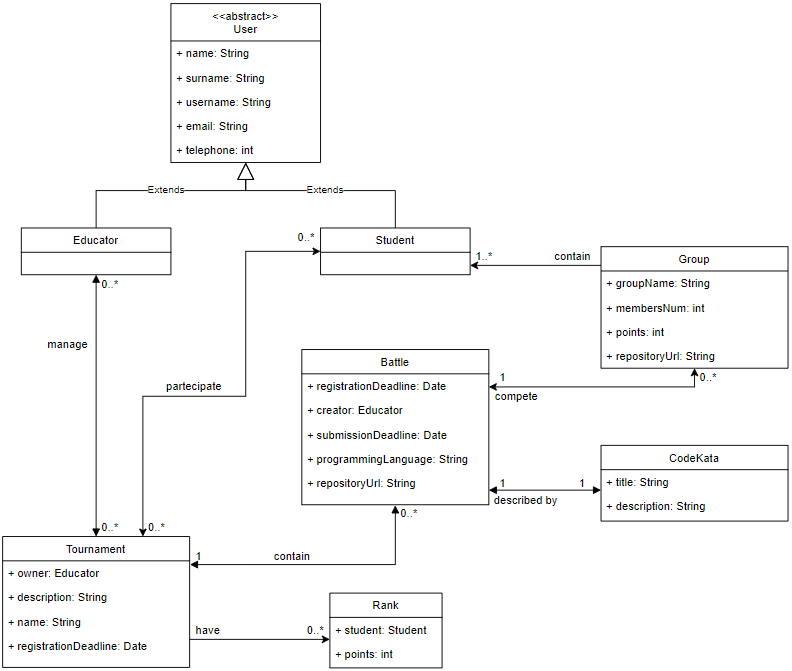
\includegraphics[width=0.9\linewidth]{images/class.png}
    \end{figure}
    The main elements of the UML Class diagram presented above are: 
    \begin{itemize}
        \item \textit{Educator}: every \textit{Educator} has a name, surname, username, email, and telephone. 
            The username must be unique. 
            The \textit{Educator} is able to manage multiple \textit{Tournament}. 
        \item \textit{Student}: every \textit{Student} has a name, surname, username, email, and telephone. 
            The username must be unique. 
            The \textit{Student} is able to partecipate in multiple \textit{Battle}, that is part of a certain \textit{Tournament}. 
            The \textit{Student} is part of a \textit{Group} for a given \textit{Battle}.     
        \item \textit{Group}: every \textit{Student} that partecipate in a \textit{Battle} must set up a group with the number of \textit{Student} fixed by the rules. 
            Each group is created for a specific \textit{Battle} within a \textit{Tournament}. 
            Different \textit{Battle} within the same \textit{Tournament} may have different \textit{Group}. 
            The \textit{Student} that creates a group have to set up a groupName. 
            The system automatically set the groupId (univoque) and the membersNum based on the \textit{Battle}'s rule. 
            It has a relation with \textit{Student} and \textit{Battle}, since it is formed by one or more \textit{Student} and is created in the context of a specific \textit{Battle}. 
            It has also a relation with \textit{GroupRepository} since every \textit{Group} needs a repository to partecipate in a given \textit{Battle}. 
        \item \textit{GroupRepository}: this class contains the URL of the repository associated to each group. 
            This is used by the system to know every repository that is subscribed to a given \textit{Battle}. 
            The system checks (after a notification by GitHub Actions) the repository and the code and updates the \textit{Rank} points. 
        \item \textit{Battle}: this class contains a single \textit{Battle} within a \textit{Tournament}.
            The \textit{Battle} has a registration and submission deadline, an univoque ID, the requested programming language, and the URL of the main repository from which users have to fork their own.
            The \textit{Battle} is created by a single \textit{Educator}, so it specifies who created it with the creator attribute. 
            Each \textit{Battle} may have multiple \textit{Group} and, consequently, multiple \textit{Student}. 
            Each battle is part of a specific \textit{Tournament} and has a \textit{CodeKata} that describes the problem. 
            Every battle has a \textit{Rank}, that updates during the \textit{Battle} itself. 
        \item \textit{CodeKata}: is the description of a problem within a \textit{Battle}. 
            It contains the name of the problem and a textual description of it. 
            Each \textit{Battle} has exactly one \textit{CodeKata}. 
        \item \textit{Tournament}: each \textit{Tournament} is created by an \textit{Educator} that becomes the owner of it. 
            It has a unique ID, a textual description on the general topic, and the name. 
            It also has a deadline for the whole \textit{Tournament}. 
            The manage relation indicates the \textit{Educator}s that manage the \textit{Tournament} in cooperation with the owner of it. 
            The \textit{Tournament} hase a relation with \textit{Battle} and \textit{Student} it is composed by some \textit{Battle}s and one or more students are enrolled. 
            Finally, it has also a general \textit{Rank}, that specifies the rankings of all battles combined. 
        \item \textit{Rank}: it comprises a points attributes (that ranges between 0 and 100) and the group linked to this value. 
            Each \textit{Tournament} and \textit{Battle} has a list of \textit{Rank} that, ordered by the points attributes return the actual standings. 
    \end{itemize}

    \subsection{State diagrams}
    They are now presented the UML State diagrams that defines the possible states for battle and a tournament. 
    These two scenarios are analyzed as they are the core part of the whole application.
    In particular, an educator can create a tournament by setting all the rules and its battles. 
    Then the tournament has his own lifecycle shown in the diagram. 
    In each tournament there can be multiple battles. 
    At a certain point of the tournament there can be battles in different states. 
    
    \subsubsection{Battle state diagram}
    The diagram that represents the possible states of a battle is depicted below: 
    \begin{figure}[H]
        \centering
        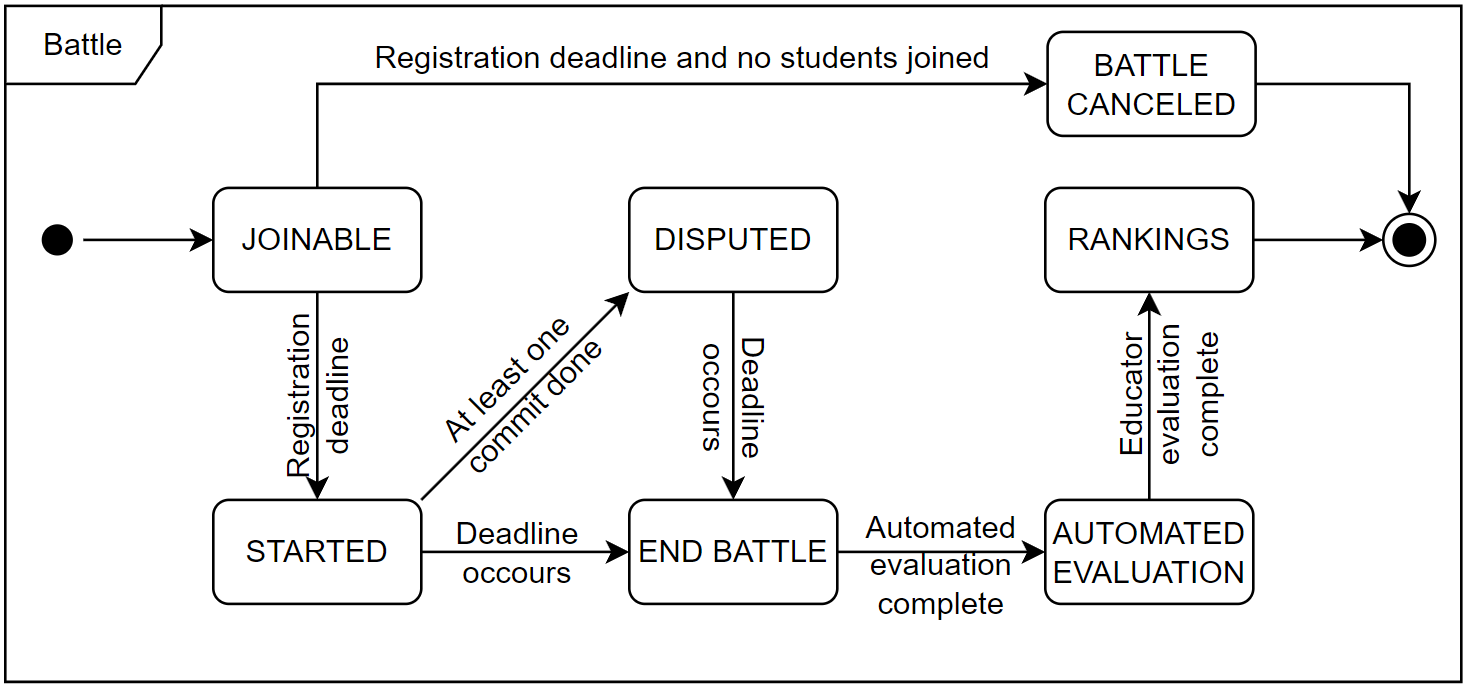
\includegraphics[width=0.75\linewidth]{images/battle.png}
    \end{figure}

    \paragraph*{Description}
    After the creation of a battle, the students enrolled in the battle's tournament can join alone or in groups (\textit{Joinable}). 
    At registratione deadline there are two possibilities: there are at least one student enrolled or there are none. 
    In the former scenario the battle starts (\textit{Started}), while in the latter the battle ends immediately without final ranking (\textit{Battle canceled0} and \textit{Final state}). 
    When the battle starts each student or group can create commits and gain points for the battle (\textit{Disputed}).
    However, when the deadline occours the battle is closed and both groups and student with and without commits are evaluated (\textit{End battle}). 
    Obviously, the groups without commits will gain zero points. 
    The solutions undergo the automated evaluation (\textit{Automated evaluation}) and then the educator's evaluation (\textit{Rankings}). 
    After all this process the final rankings are shown and the winner is revealed. 

    \subsubsection{Tournament state diagram}
    The diagram that represents the possible states of a tournament is shown below: 
    \begin{figure}[H]
        \centering
        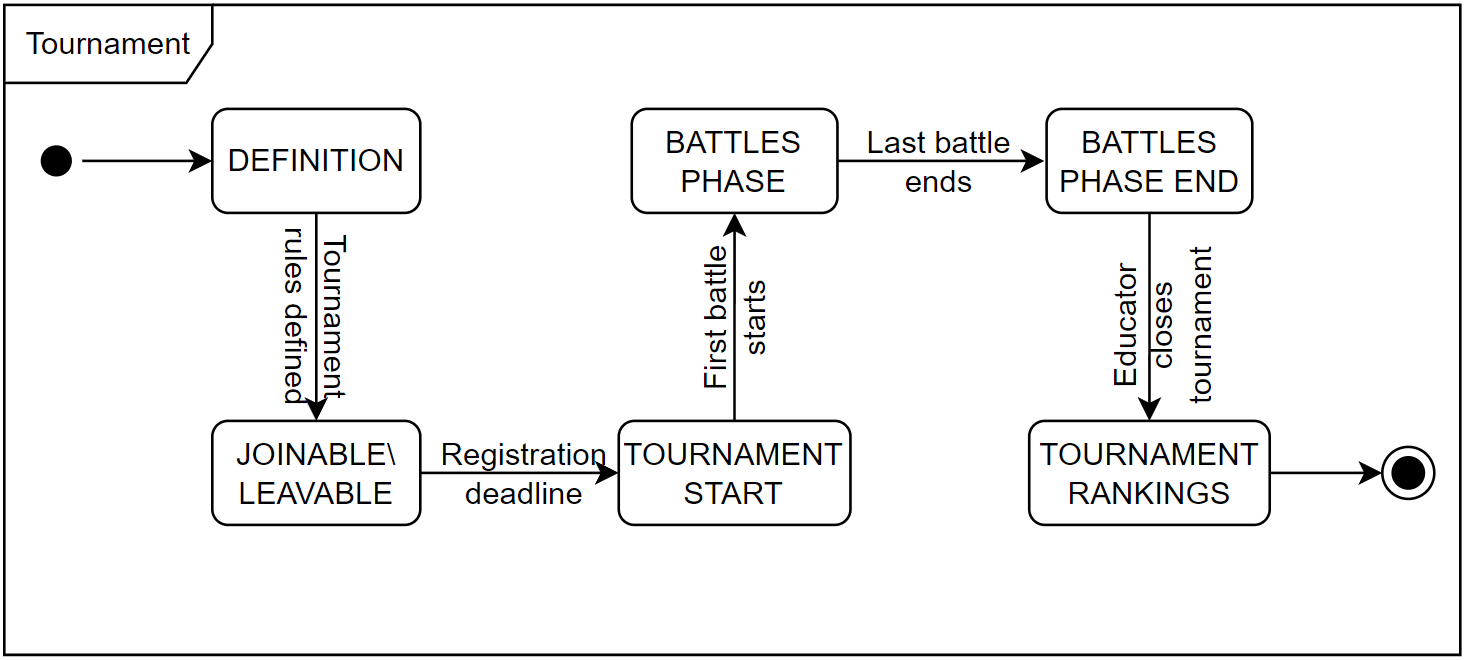
\includegraphics[width=0.75\linewidth]{images/tournament.png}
    \end{figure}

    \paragraph*{Description}
    After the creation of a tournament, the educator can invite other educator to manage it together (\textit{Definition}). 
    While doind this the educator has also to set up the rules for the tournament and the termination date (\textit{Joinable/leavable}).
    Note that the educators can create battles also after the creation of the tournament.
    When the registration deadline occours the tournament starts and students not enrolled cannot join the tournament anymore (\textit{Tournament start}). 
    After the tournament starts, the battles can also commence. 
    When the first battle starts (\textit{Battle phase}) the students can compete in the open battles and have to wait the opening date for the ones not yet stared. 
    When the last battle ends (the deadline must be anterior to the tournament ending) (\textit{Battle phase end}), it is possible to compute the scores for all the students. 
    WHen the tournament's deadline occours, the educator close the tournament itself and can finally reveal the final winner. 

    \section{Product functions}
    The functionality offered by CodeKataBattle differs based on the user that is going to interact with it. 
    Thus, the functionalities are spresented based on the user. 
    
    \subsection{Student's functionalities}
    The educator is the user that partecipates to the tournaments and the battles. 
    After the login the system must redirect the student to the page that offers the following functionalities: 
    \begin{itemize}
        \item \textit{Join tournaments}: the user must be able to access a list of opened tournament that can be joined. 
            This list has also to show if the user is eligible for the opened tournaments. 
        \item \textit{Active tournaments}: the user can view all the tournaments in which he is enrolled, with the relative termination dates and the active battles within it. 
        \item \textit{Tournament details}: the user can view the details of a tournament. 
            It can see the status of all battles and the relative rankings. 
        \item \textit{Battles details}: the user can view the details of each battle. 
            The details consist, if the battle is open, in the problem description and test files. 
            It can check the catual ranking, the points it has received, and the details about commits it has done. 
            If the battle is closed it can see the final ranking.
            If the battle is not yet open he can view only the topics and the other user enrolled, but not the problem itself. 
    \end{itemize}

    \subsection{Educator's functionalities}
    The educator is the user that manages the tournaments and the battles. 
    After the login the system must redirect the educator to the page that offers the following functionalities: 
    \begin{itemize}
        \item \textit{Create tournaments}: the user can create a new tournament by setting the rules and adding other educator to help it manage the competition. 
            After setting up collaborators and rules, it (and the collaborators) can add battles to the tournament. 
            When this phase ends the tournament is ready to be seen by the students. 
        \item \textit{Add battle}: the user must have the possibility to add a new battle also after the creation of the tournament. 
            This functionality allow, by selecting a managed tournament, to create a new battle with all the rules and add it to the tournament. 
        \item \textit{Manage tournament}: after the creation of the tournament the educator can check the status until the end and close it when the time expires. 
        \item \textit{Manage battle}: when a battle in a certain managed tournament is active the user can see the actual rankings and the commit status of each participant. 
            If specified by the rules, when the time expires he must check the final submissions for each group and assign points based on the quality and finally close the battle. 
            If the manual check is not in the rules he can directly close the battle when the time expires. 
    \end{itemize}

    \section{User characteristics}
    The platform accommodates interaction from two user categories: students and educators. The initial user category engages in Code Kata tournaments, while educators, 
    on the other hand, serve as the organizers of these tournaments.
    
    \subsection{Student}
    The student, as an individual aiming to secure victory in a specific battle, may need to either join an existing team or establish one with fellow students, considering that each battle has a predetermined group size. \\
    In particular, a student requires access to the following features within the system:
    \begin{itemize}
        \item Student login.
        \item Personalized user interface. 
        \item Access to the list of available tournaments.
        \item The ability to join a desired tournament if it's open for registration.
        \item Capability to create and join groups.
        \item Access to the GitHub repository link for a specific tournament.
        \item Access to both interim and final tournament rankings.
    \end{itemize}

    \subsection{Educator}
    The educator's role encompasses the creation and management of tournaments, with the potential involvement of other educators designated by the tournament's owner, who is typically the initiating educator. 
    All educators should possess the capability to create code Katas for the tournaments they manage and provide additional points for evaluation. \\
    To facilitate these responsibilities, educators need access to the following features within the system:
    \begin{itemize}
        \item Educator login. 
        \item Personalized user interface. 
        \item Access to a list of tournaments under their management.
        \item The possibility to create new tournaments. 
        \item The ability to create new battles with customized rules. 
        \item Within a managed tournament: 
            \begin{itemize}
                \item The option to invite other educators to participate. 
                \item The capability to add new code Katas.
                \item The authority to close the tournament.
                \item The ability to assign extra points if specified in the battle rules.
            \end{itemize}
        \item Access to the GitHub repository for every student in the active tournament.
        \item Access to both interim and final tournament rankings.
    \end{itemize}

    \section{Assumptions, dependencies and constraints}

    \subsection{Domain assumptions}
    The domain assumptions that we have to make are: 
    \begin{itemize}
        \item All the users must regiter with an email associated with a GitHub account. 
        \item The educators must not commit on student's repositories. 
        \item The students do not share their code with students of other groups. 
        \item A student submits a code that is not malicious. 
        \item Every user register itself to the website with the right role (student or educator).
        \item GitHub and the API always works correctly. 
        \item The test cases uploaded by the educators are correct. 
        \item The CodeKata problem proposed has a solution. 
        \item The students fork the repository and set up an automated workflow GitHub Actions. 
    \end{itemize}

    \subsection{Dependencies}
    The dependencies that we have to make are: 
    \begin{itemize}
        \item The system requires an internet connection to retrieve all the data. 
        \item The system will use an external API to interact with GitHub to check for commits and to create the repositories.
        \item The system will use an external API to send notifications to the user. 
    \end{itemize}

    \subsection{Constraints}
    The system shall be compliant to local laws and regulations, in particular users data should be treated according to the GDPR. 
    The user must be able to retrive the personal data given to the site ache time he needs them. 
    The data collected in the registration phase must be the strictly necessary ones. \\
    All information given from the user must be encrypted to protect them from malicious users. \\
    The APIs used by the application must be choosen based on security and reliability.

\chapter{Specific requirements}
    \section{External interface requirements}
        In this section are presented all the interfaces required by the system to work as intended. 

        \subsection{User interfaces}
        The platform will be implemented via a website that present a different interface based on the user type. \\
        The website interface will be modified based on the type of hardware used (mobile or personal computer). 

        \subsubsection{Welcome page} 
        This is the page that is shown when the user is not registered or logged in. 
        There is a brief description of the website and two buttons to let the user enter in the system. 
        \begin{figure}[H]
            \centering
            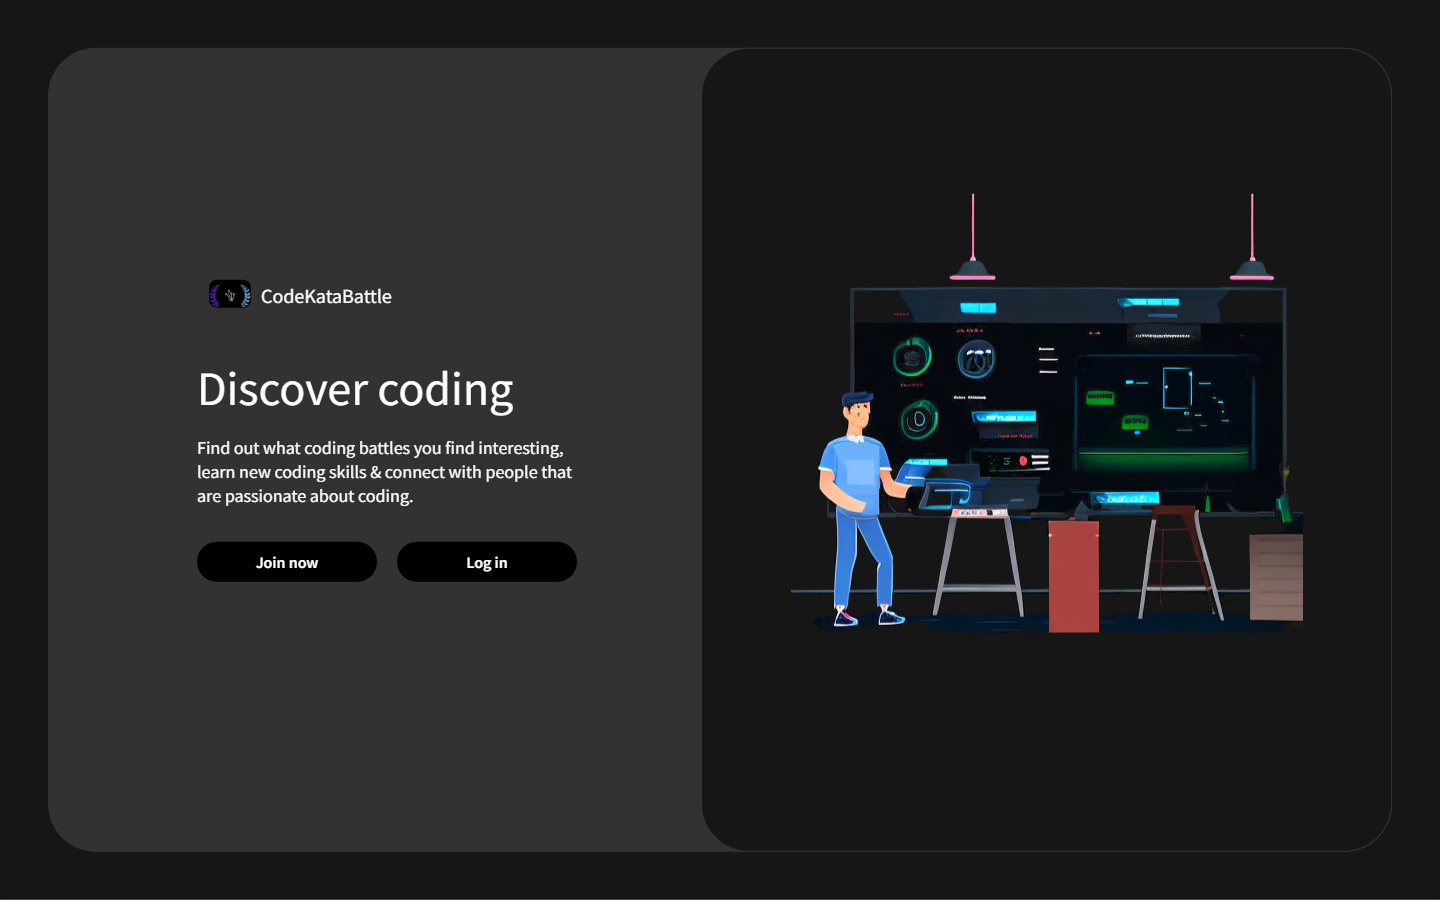
\includegraphics[width=0.8\linewidth]{images/welcome.png}
        \end{figure}

        \subsubsection{Sign in page} 
        In this page the user can select the corresponding role on the left and add the information required to register.
        After completing all the information the user must click on the sign-in button to finally register.
        \begin{figure}[H]
            \centering
            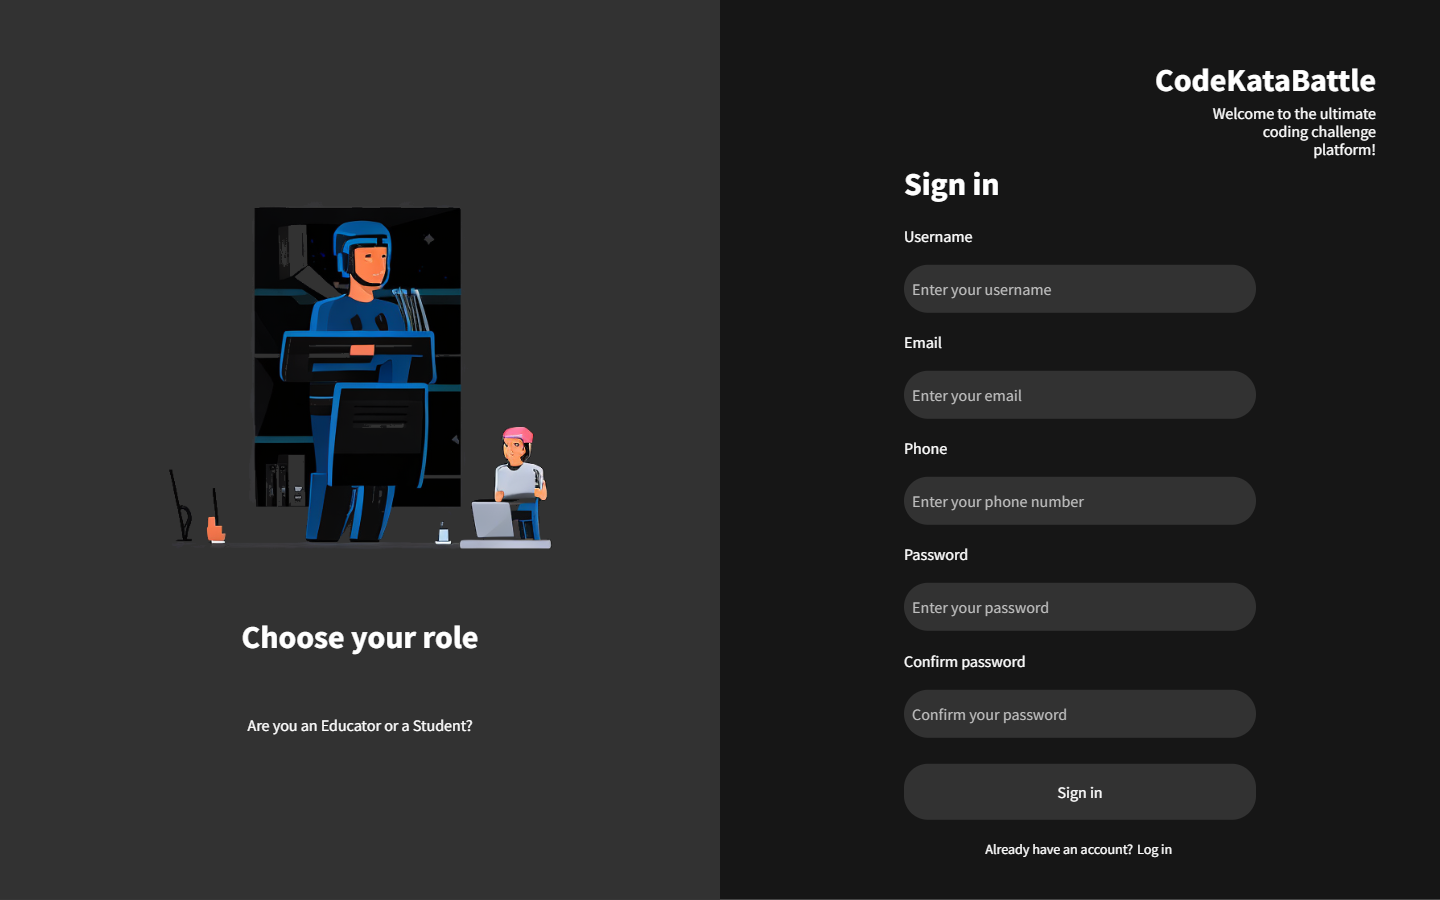
\includegraphics[width=0.8\linewidth]{images/sign_in.png}
        \end{figure}

        \subsubsection{Login page} 
        In this page the user must select the role, and insert the credentials if already registered in the system. 
        If the credentials are correct the user can access the functionalities associated with him. 
        \begin{figure}[H]
            \centering
            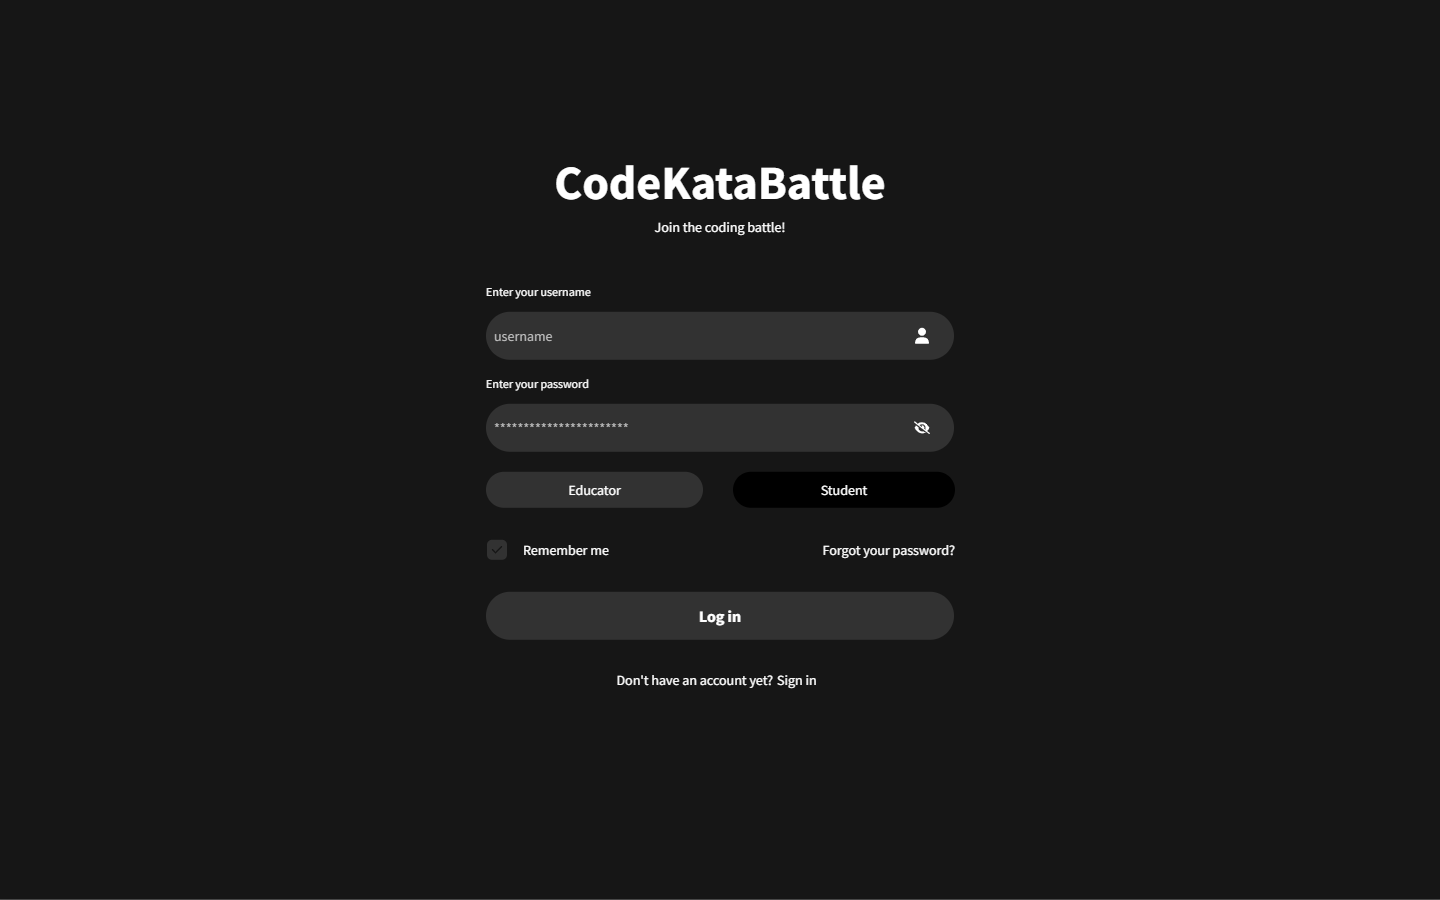
\includegraphics[width=0.8\linewidth]{images/log_in.png}
        \end{figure}

        \subsubsection{Home page} 
        The home page shows all active tournament and the tournament checked before by the current user. 
        If the home page is accessed by the Educator the buttons are for viewing details instead of joining the tournament. 
        \begin{figure}[H]
            \centering
            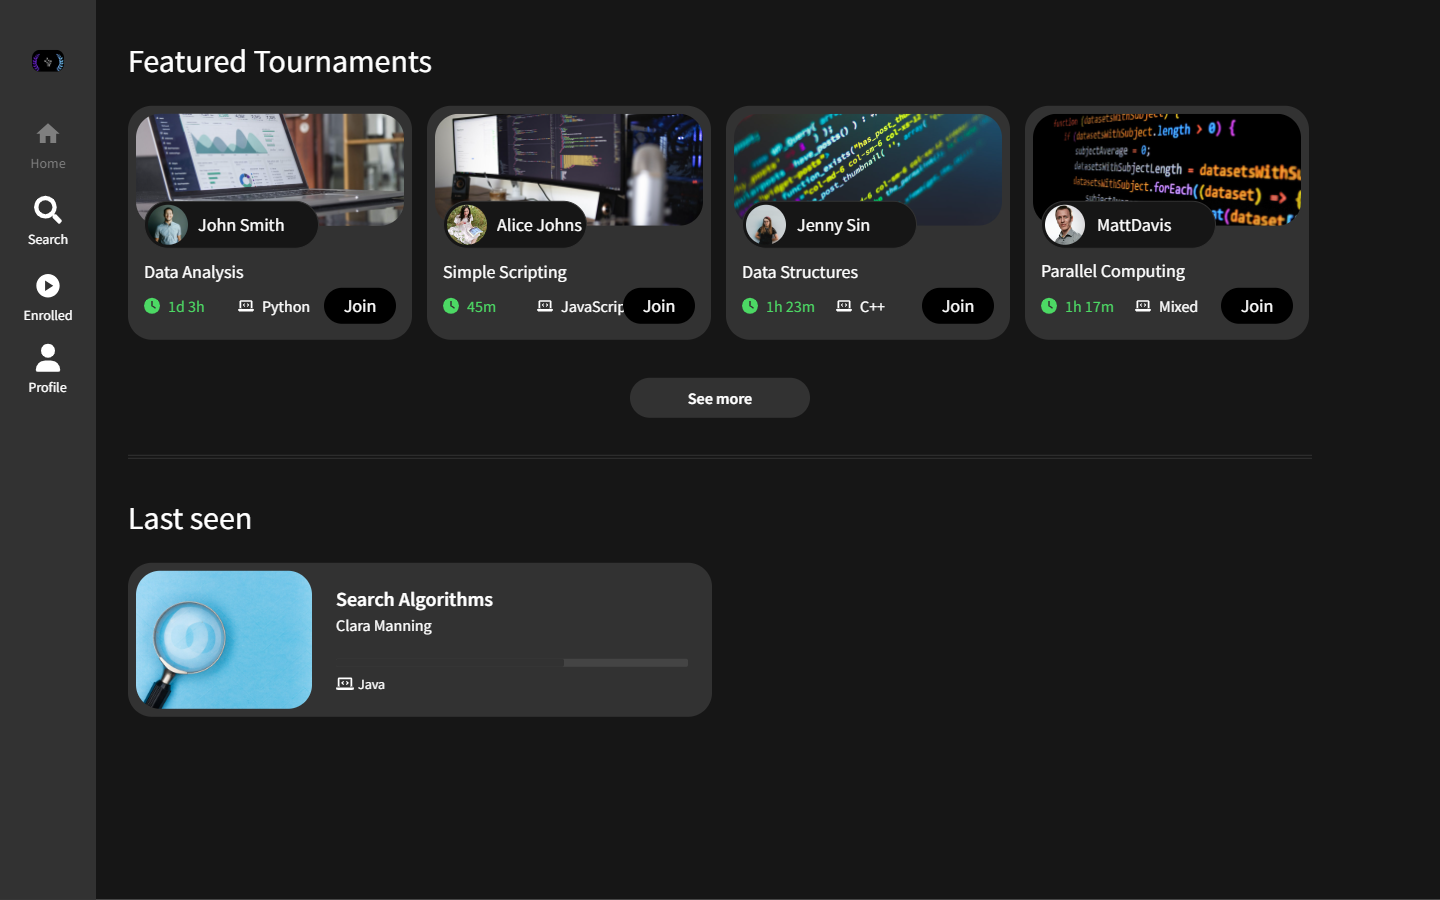
\includegraphics[width=0.8\linewidth]{images/home.png}
        \end{figure}

        \subsubsection{Profile page} 
        In the profile page the users can modify the personal description and the image related to the account. 
        Other functionalities for the Student are: check active tournaments, check personal statistics and view the details of ended tournament in which the student partecipated.
        The Educator has the same page (without statistics) and the tournament listed are the one who he is managing. 
        \begin{figure}[H]
            \centering
            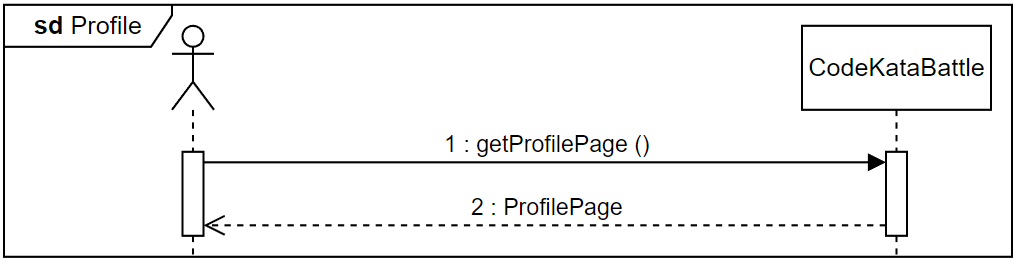
\includegraphics[width=0.8\linewidth]{images/profile.png}
        \end{figure}

        \subsubsection{Search page} 
        In this page the user can filter by choosing the desired language or by name. 
        The first action can be done by selecting one of the button below "Languages", while the second is done with the bar at the top of the page. 
        Also in this page the join buttone becomes a details button for the Educator. 
        Finally, at the bottom of the page there is a section with recommendend battles based on the previous researches.
        \begin{figure}[H]
            \centering
            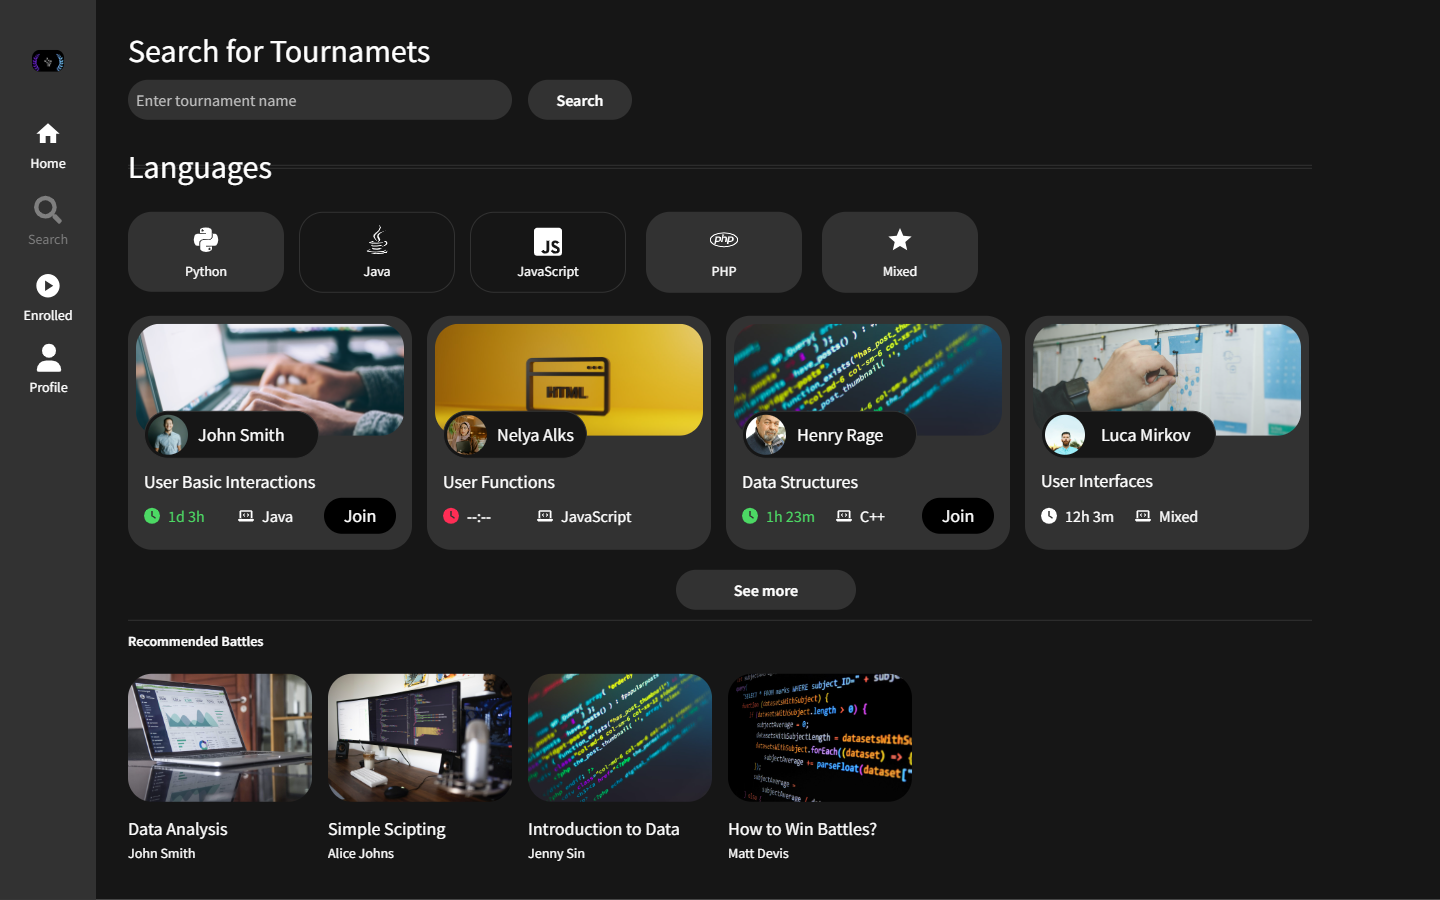
\includegraphics[width=0.8\linewidth]{images/search.png}
        \end{figure}

        \subsubsection{Enrolled page} 
        This page is only for Students. 
        Here they can view the active tournaments where they are enrolled, and check the details (the battles within a tournament) and the current leaderboard.
        \begin{figure}[H]
            \centering
            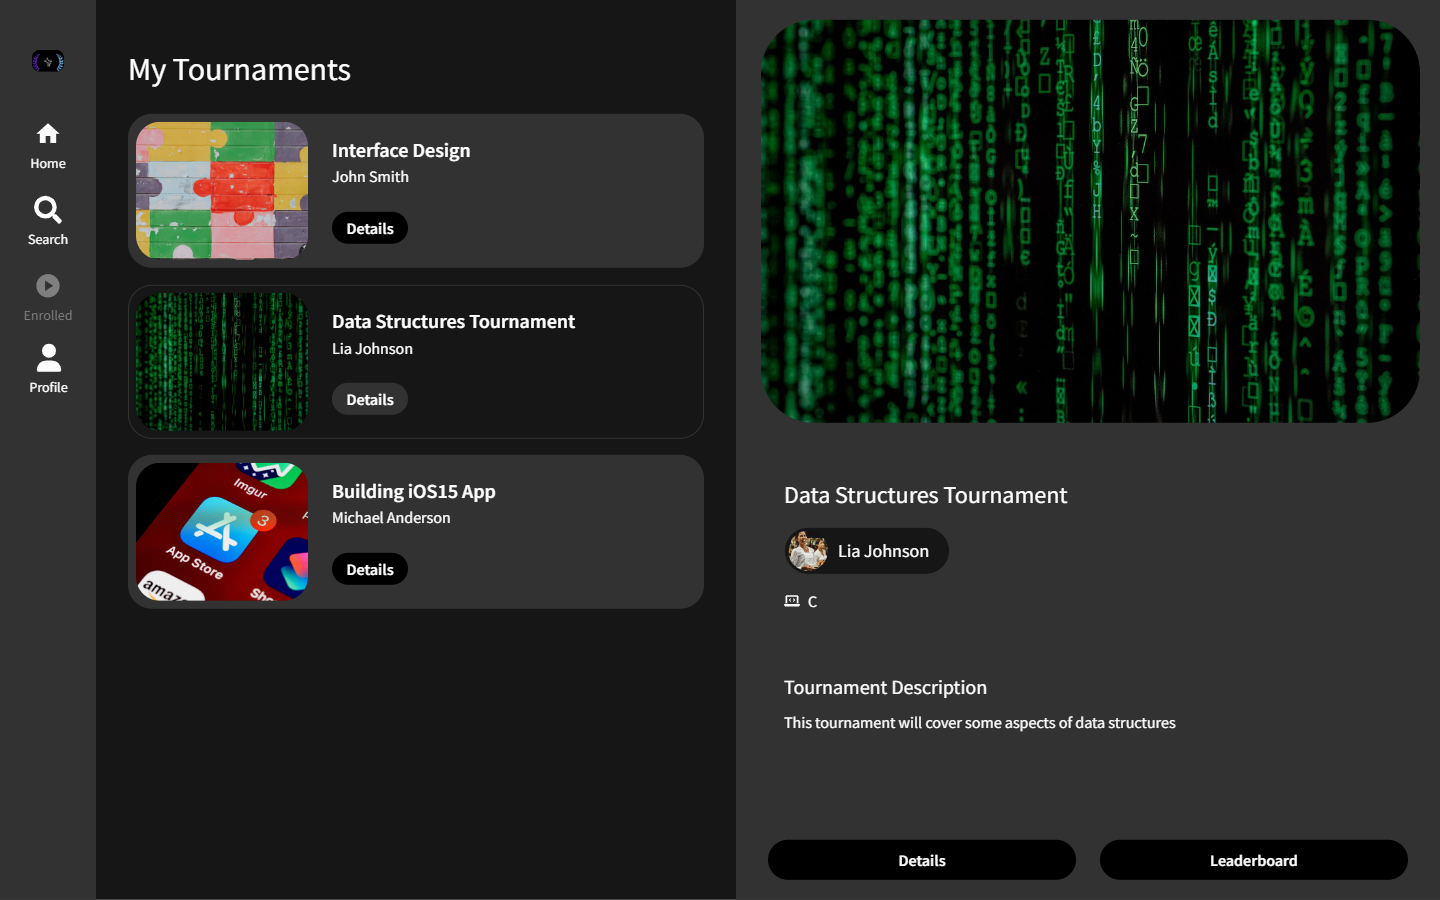
\includegraphics[width=0.8\linewidth]{images/enrolled.png}
        \end{figure}

        \subsubsection{Tournament details page} 
        This page is for the Student and shows all the battles within a tournament. 
        Here the student can join the single battles with a group made of one or more people. 
        \begin{figure}[H]
            \centering
            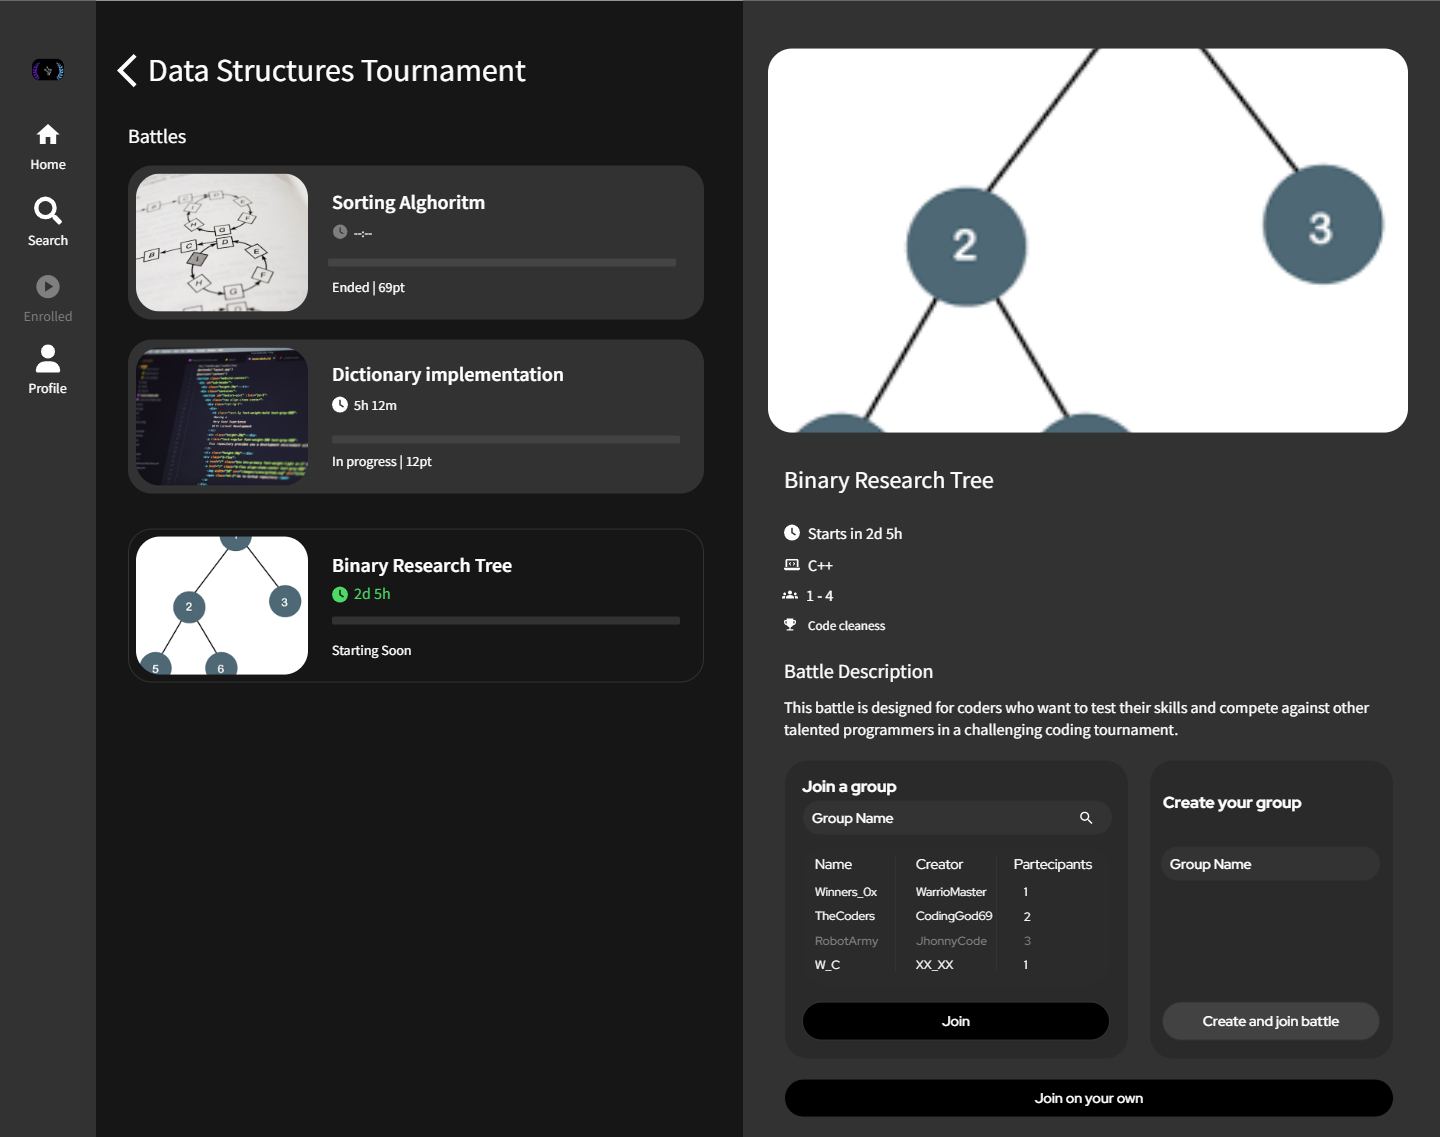
\includegraphics[width=0.8\linewidth]{images/tournament_details.png}
        \end{figure}

        \subsubsection{Leaderboard page} 
        The leaderboard page shows the current ranking of the tournament selected with the details button in other pages. 
        \begin{figure}[H]
            \centering
            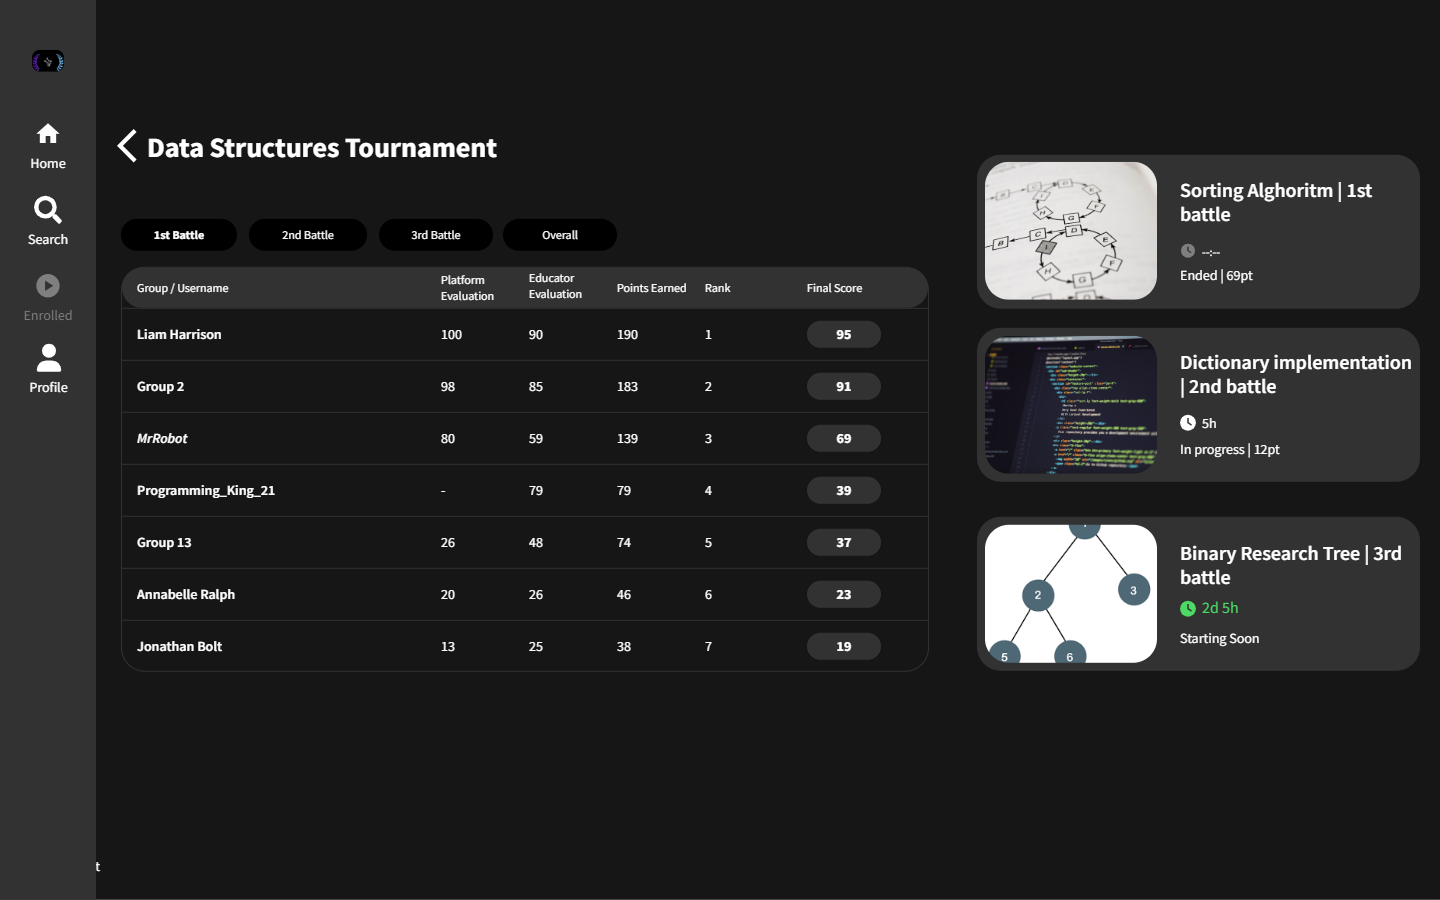
\includegraphics[width=0.8\linewidth]{images/leaderboard.png}
        \end{figure}

        \subsubsection{Create tournament page} 
        In this page the Educator can set all the items needed to create a new tournament. 
        \begin{figure}[H]
            \centering
            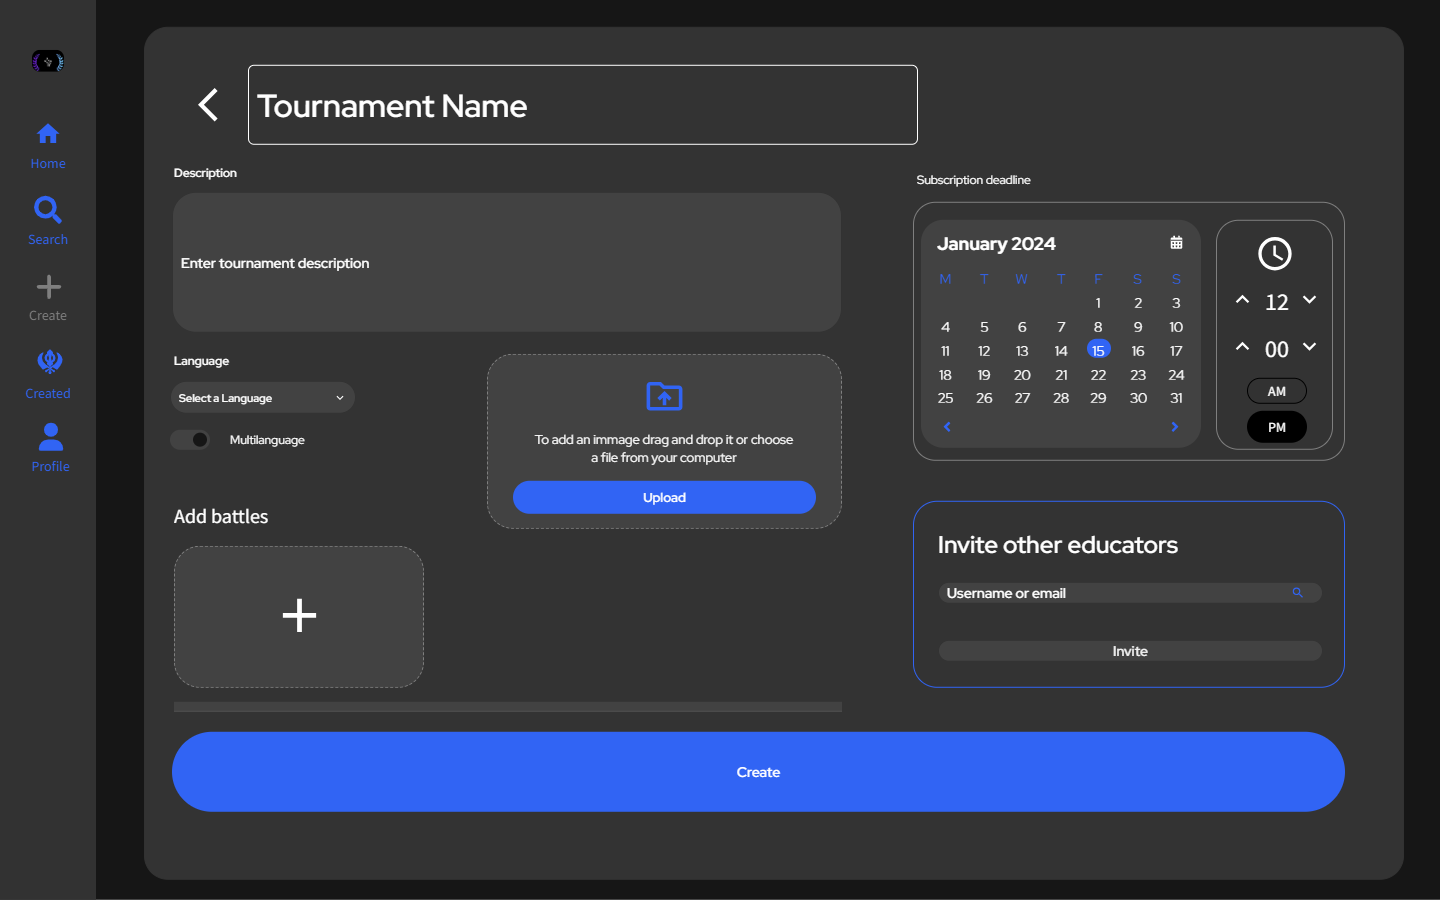
\includegraphics[width=0.8\linewidth]{images/create_tournament.png}
        \end{figure}

        \subsubsection{Create battle page} 
        In this page the Educator can set all the items needed to create a new battle within a tournament. 
        \begin{figure}[H]
            \centering
            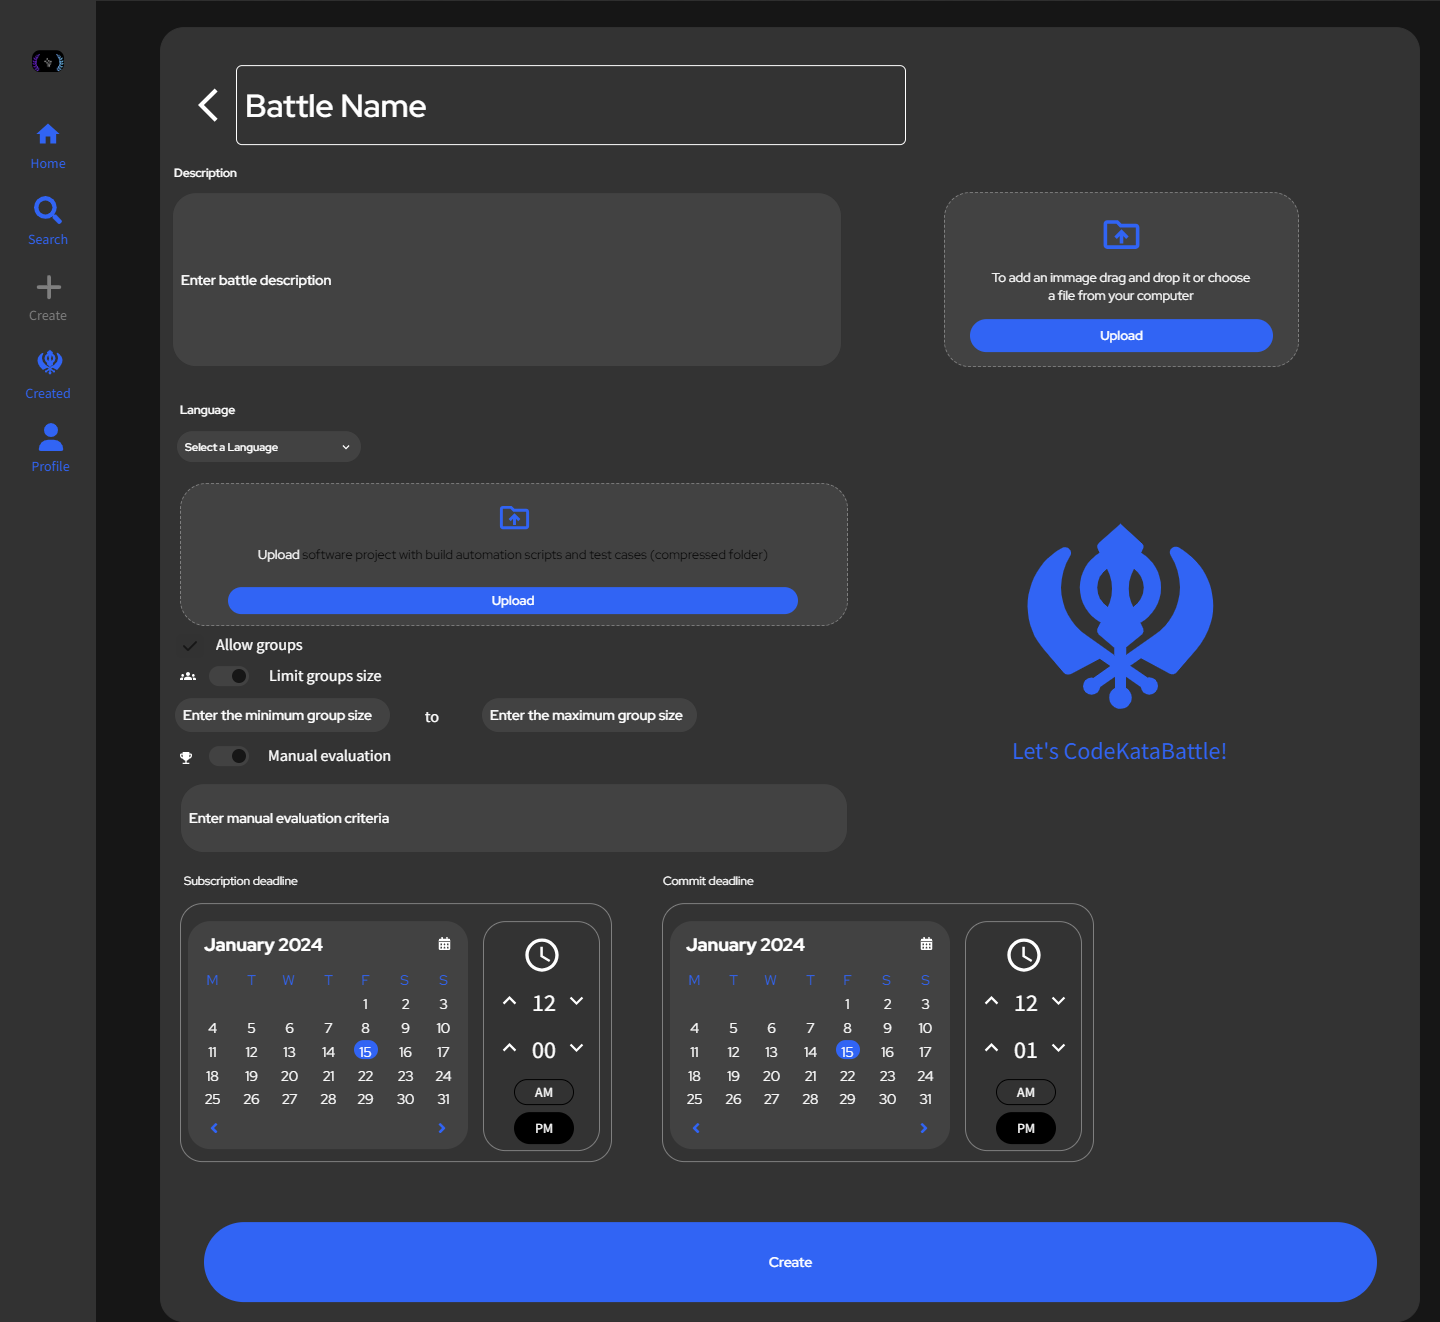
\includegraphics[width=0.75\linewidth]{images/create_battle.png}
        \end{figure}

        \subsubsection{Manage tournament page} 
        In the manage tournament page the Educator can select the tournament that he manages and modify them by addin a battle, invite collaborators or close. 
        It can also check the shared tournaments (where he is not the owner, but a collaborator). 
        \begin{figure}[H]
            \centering
            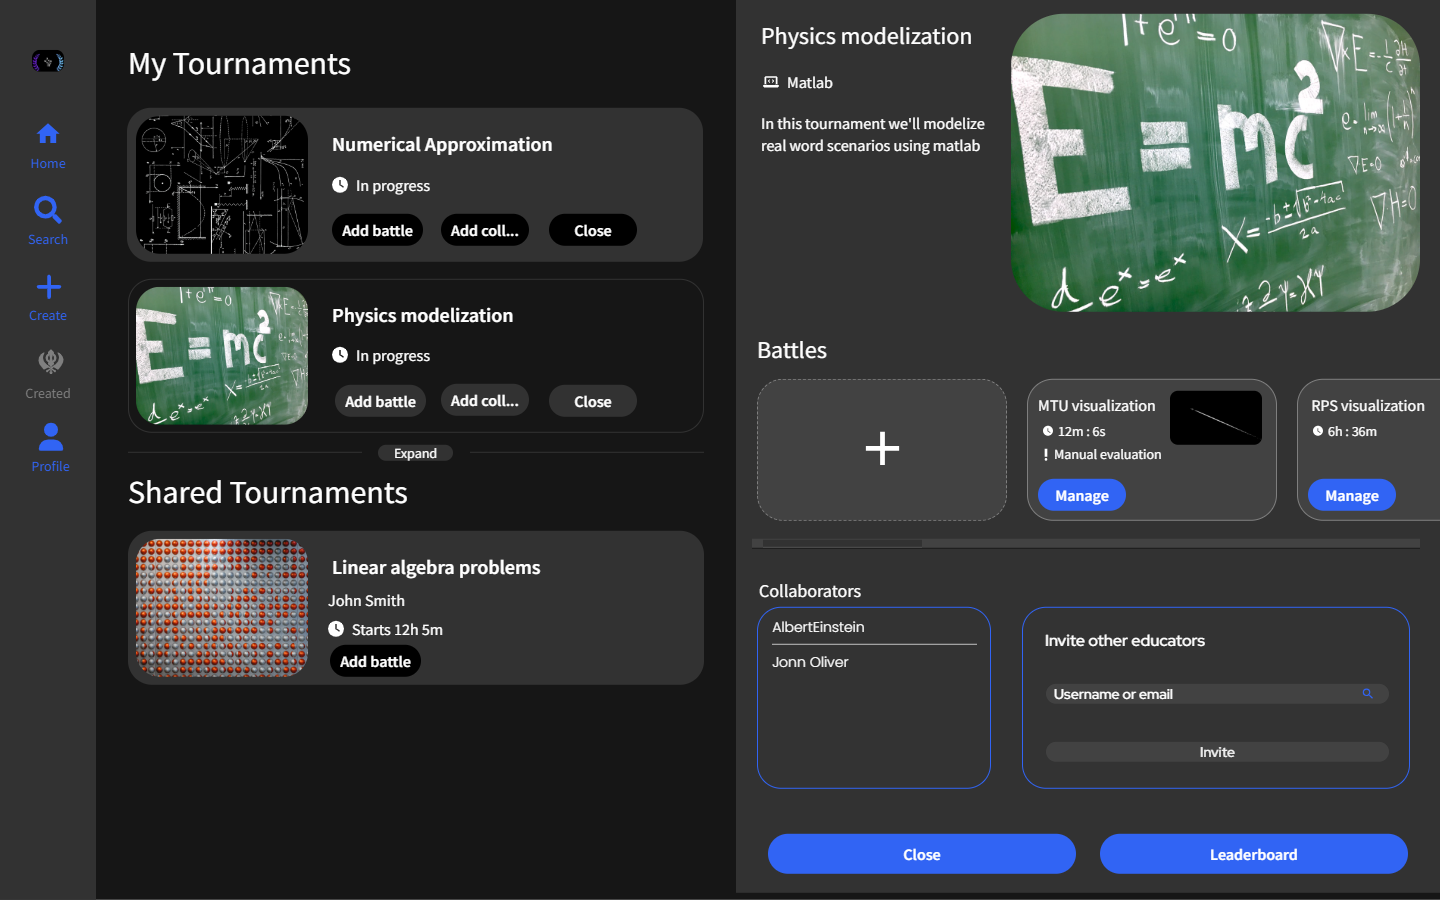
\includegraphics[width=0.8\linewidth]{images/manage_tournament.png}
        \end{figure}

        \subsubsection{Manage battle page} 
        In this page the Educator can check the status of the battles within a specific tournament. 
        Here, he can check the final rankings and add the manual evaluation when needed.
        \begin{figure}[H]
            \centering
            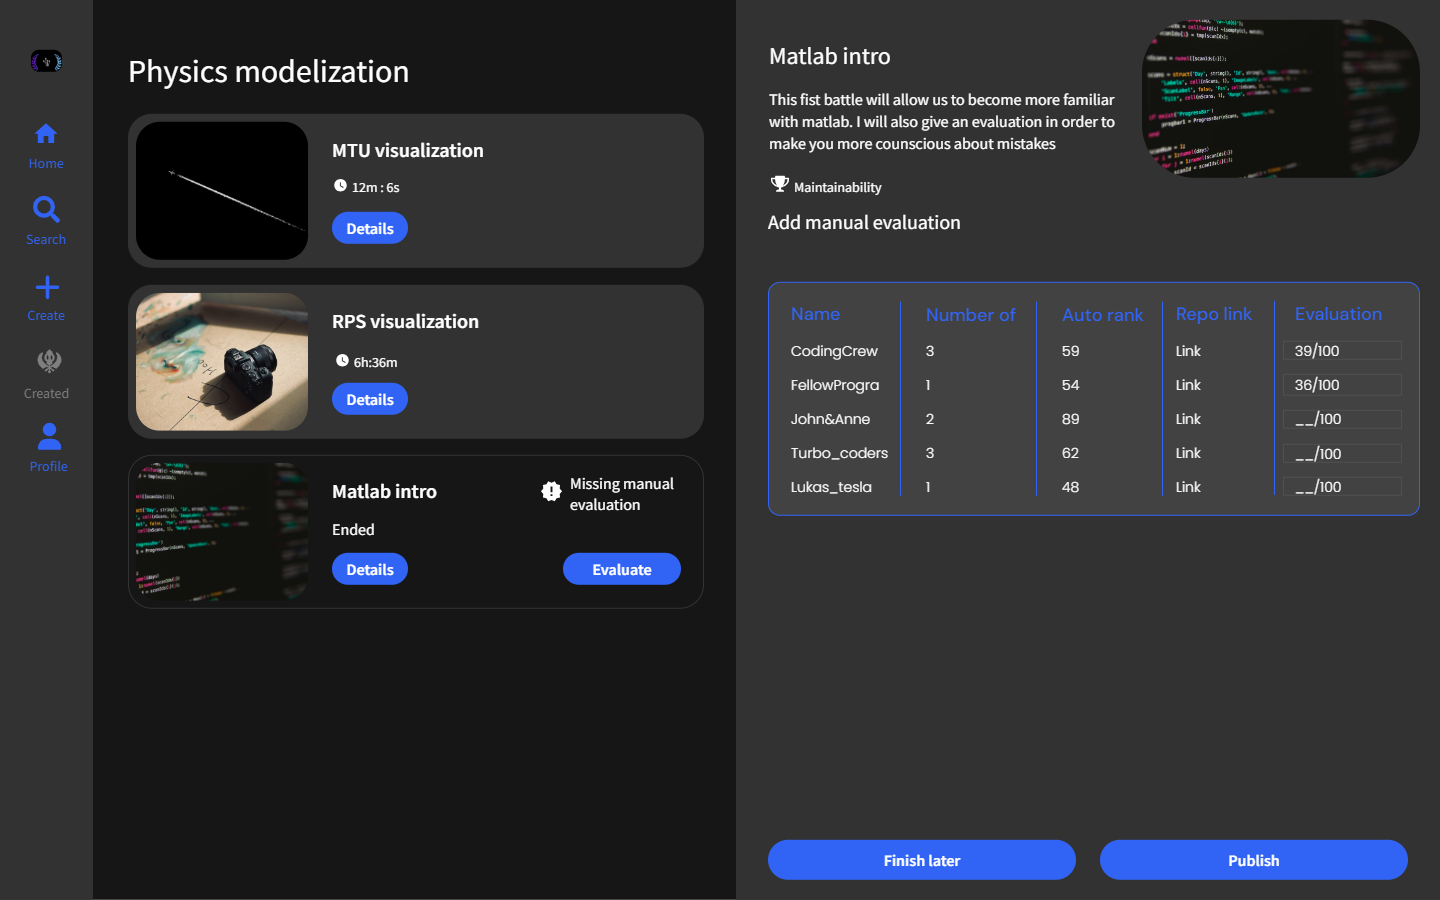
\includegraphics[width=0.8\linewidth]{images/manage_battle.png}
        \end{figure}

        \subsection{Hardware interfaces}
        Both user must have a mobile device or a personal computer. 
        Since the system will be implemented as a website the personal computer will be a better device for visualize better all the information. \\
        Additionaly, the challenge is to solve some problems using programming language, so the personal computer is necessary to compete (it is possible also with mobile devices but certainly more difficult). 

        \subsection{Software interfaces}
        The system is a web application. 
        Thus, the only software needed for both users is a modern web browser. 

        \subsection{Communication interfaces}
        To work as intendend the system requires a reliable internet connection. 
        The backend of the application will expose a unified RESTful API. 
        This API is used to communicate with all users using HTTPS and TCP/IP protocols. \\
        Furthermore, the system uses other two application program interfaces to ensure all its functionalities: 
        \begin{itemize}
            \item Create a repository: CodeKataBattle needs to interact with GitHub in order to create a repository for each group partecipating to starting battles. 
            \item Check repositories commits: CodeKataBattle needs to interact with the repositories linked to active battles in order to check all the new commits. 
            \item Notification: CodeKataBattle needs to be able to send notification to the user to alert the users about important facts (e.g., the start or the end of a battle). 
        \end{itemize}

    \section{Functional Requirements}
        Initially we show the possible use cases for the interaction between the user and the application with the relative description and use case diagram. 
        In the second part we list all the functional requirements as a mapping between the goals and the defined use cases. 

        \subsection{Use case diagrams}
        An unregistered user must be able to sign up. 
        The registration phase is different according to the role of the user. 
        If it is a student it has to get the corresponding functionalities (i.e., partecipate in tournaments). 
        If it is an educator it has to get the corresponding functionalities (i.e., create and manage tournaments). 
        The corresponding Use Case Diagrams are shown below: 
        \begin{figure}[H]
            \centering
            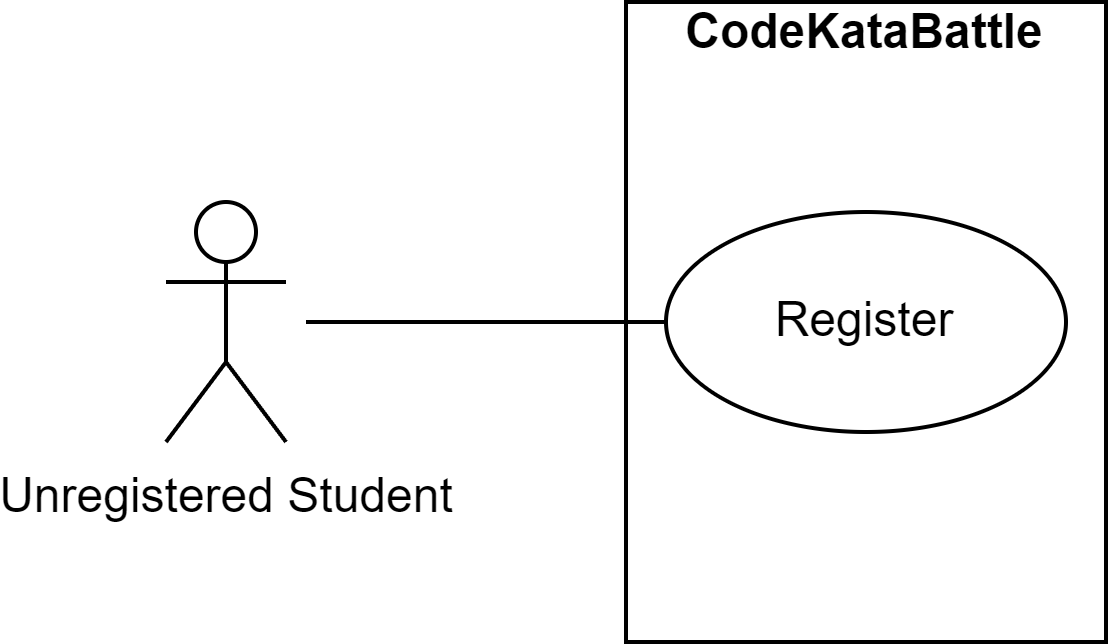
\includegraphics[width=0.5\linewidth]{images/unregisteredstud.png}
            \caption{Use Case diagram for unregistered student}
        \end{figure}
        \begin{figure}[H]
            \centering
            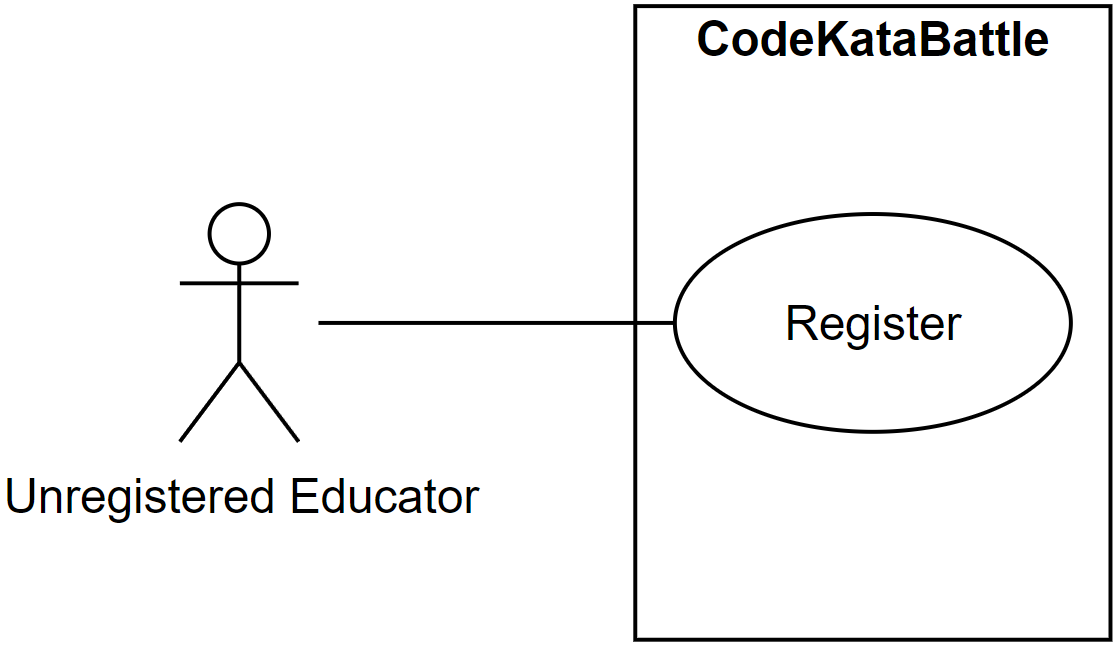
\includegraphics[width=0.5\linewidth]{images/unregistereded.png}
            \caption{Use Case diagram for unregistered educator}
        \end{figure}
        Now, we analyze all the functionalities needed for both the students and the educators after the registration in the fllowing two Use Case diagrams: 
        \begin{figure}[H]
            \centering
            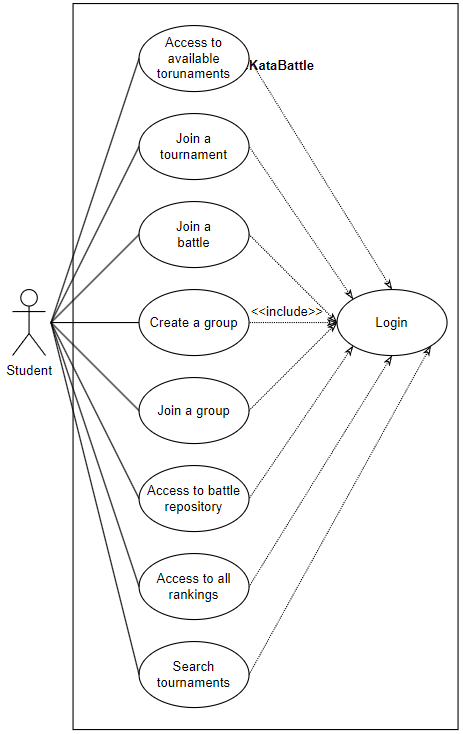
\includegraphics[width=0.65\linewidth]{images/stud.png}
            \caption{Use Case diagram for unregistered educator}
        \end{figure}
        \begin{figure}[H]
            \centering
            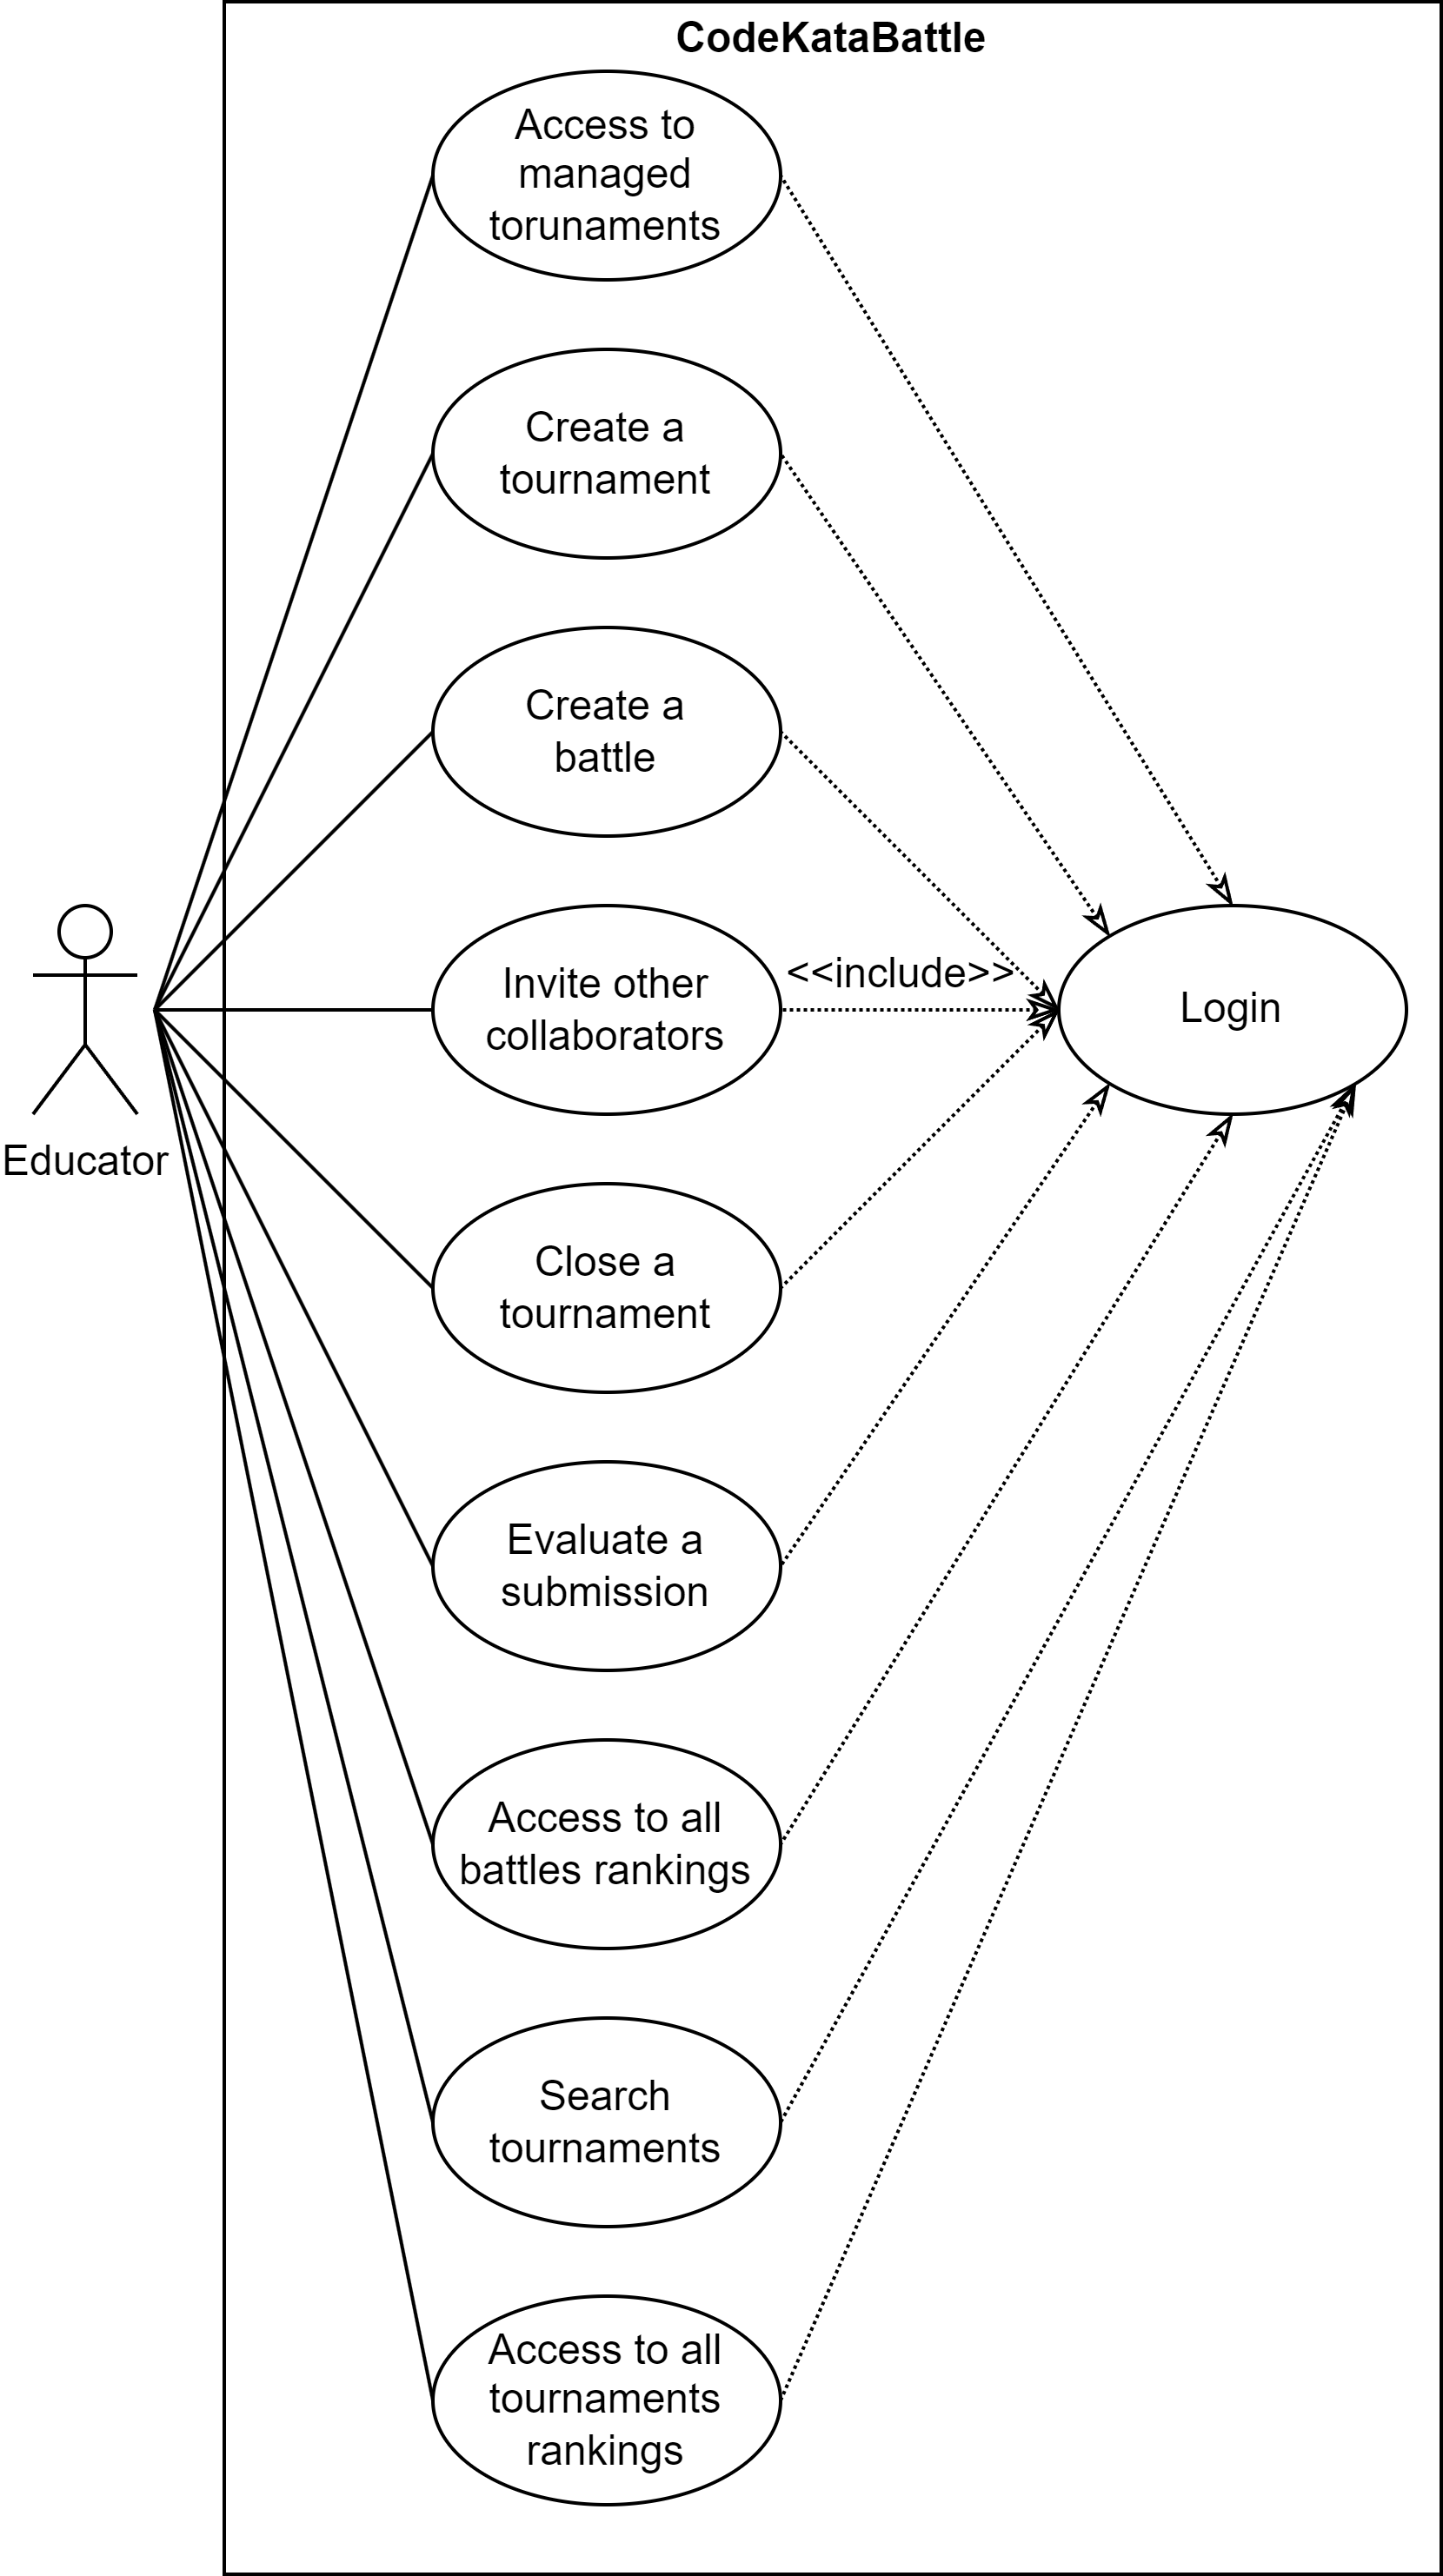
\includegraphics[width=0.65\linewidth]{images/ed.png}
            \caption{Use Case diagram for unregistered educator}
        \end{figure}

        \subsection{Use cases}
        % usecase for the registration of students
        \usecase{}
        {\arabic{useCase}\stepcounter{useCase}}
        {Student registration}
        {Student}
        {The actor clicks on the register button}
        {
        \begin{enumerate}
            \item The actor requires the sign-in page by clicking the join now button in the welcome page
            \item The system shows the sign-in page to the actor
            \item The actor inserts required personal information and sends it to the system
            \item The system processes the information and shows a success message redirecting the user to the login page
        \end{enumerate}
        }
        {The actor is registered correctly, and the login page is displayed}
        {
        \begin{itemize}
            \item An already existing username, email or phone number are submitted
            \item A required registration field is missing or invalid when the form is submitted
        \end{itemize}
        }
        {In case of exception the system will notify user with a human-readable message; the system is not able to check if the correct role was selected}

        % usecase for the registration of educators
        \usecase 
        {\begin{figure}[H]\centering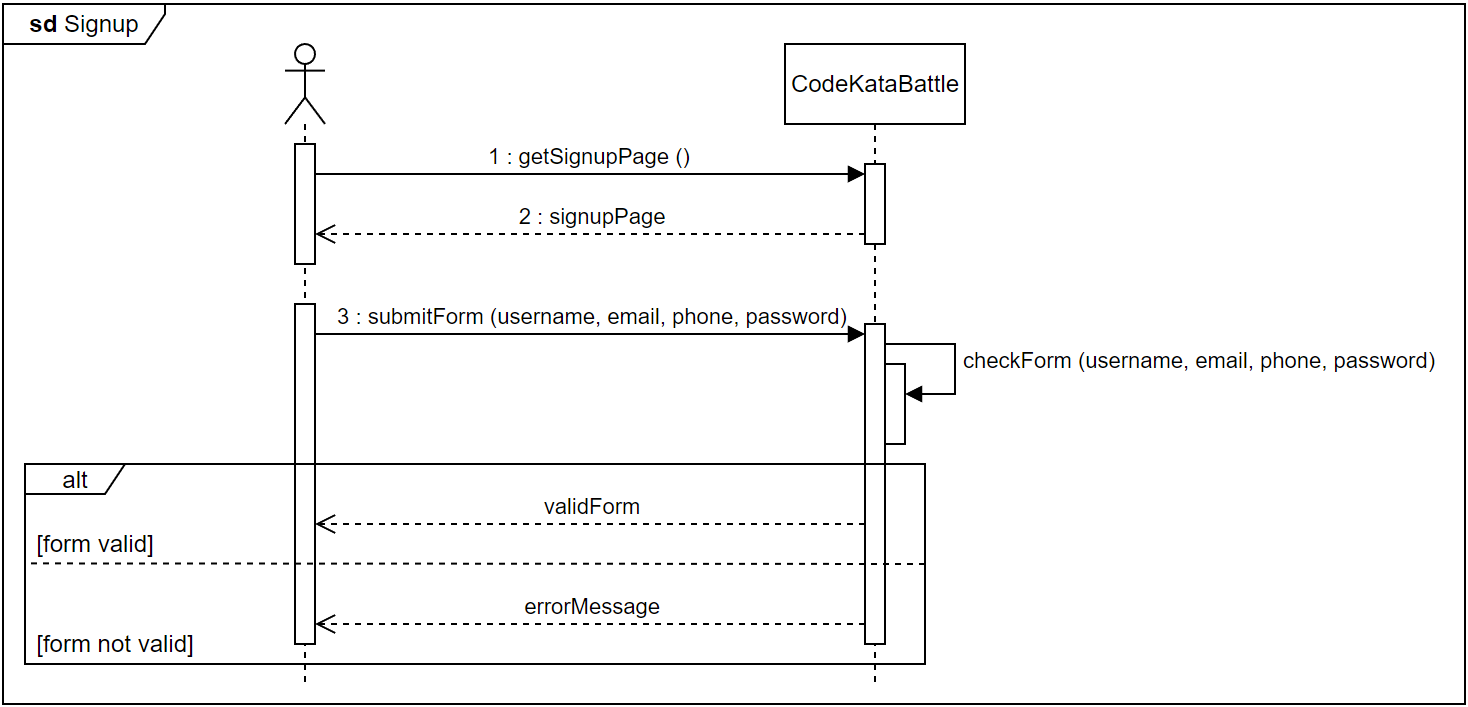
\includegraphics[width=0.9\linewidth]{images/signup.png}\end{figure}}        
        {\arabic{useCase}\stepcounter{useCase}}
        {Educator registration}
        {Educator}
        {The actor clicks on the sign-in button}
        {
        \begin{enumerate}
            \item The actor requires the sign-in page by clicking the join now button in the welcome page
            \item The system shows the sign-in page to the actor
            \item The actor inserts required personal information and sends it to the system
            \item The system processes the information and shows a success message redirecting the user to the login page
        \end{enumerate}
        }
        {The actor is registered correctly, and the login page is displayed}
        {
        \begin{itemize}
            \item An already existing username, email or phone number are submitted
            \item A required registration field is missing or invalid when the form is submitted
        \end{itemize}
        }
        {In case of exception the system will notify user with a human-readable message; the system cannot check if the right role is select during registration}

        % usecase (Student, Educator) for the login of both students and educators 
        \usecase
        {\begin{figure}[H]\centering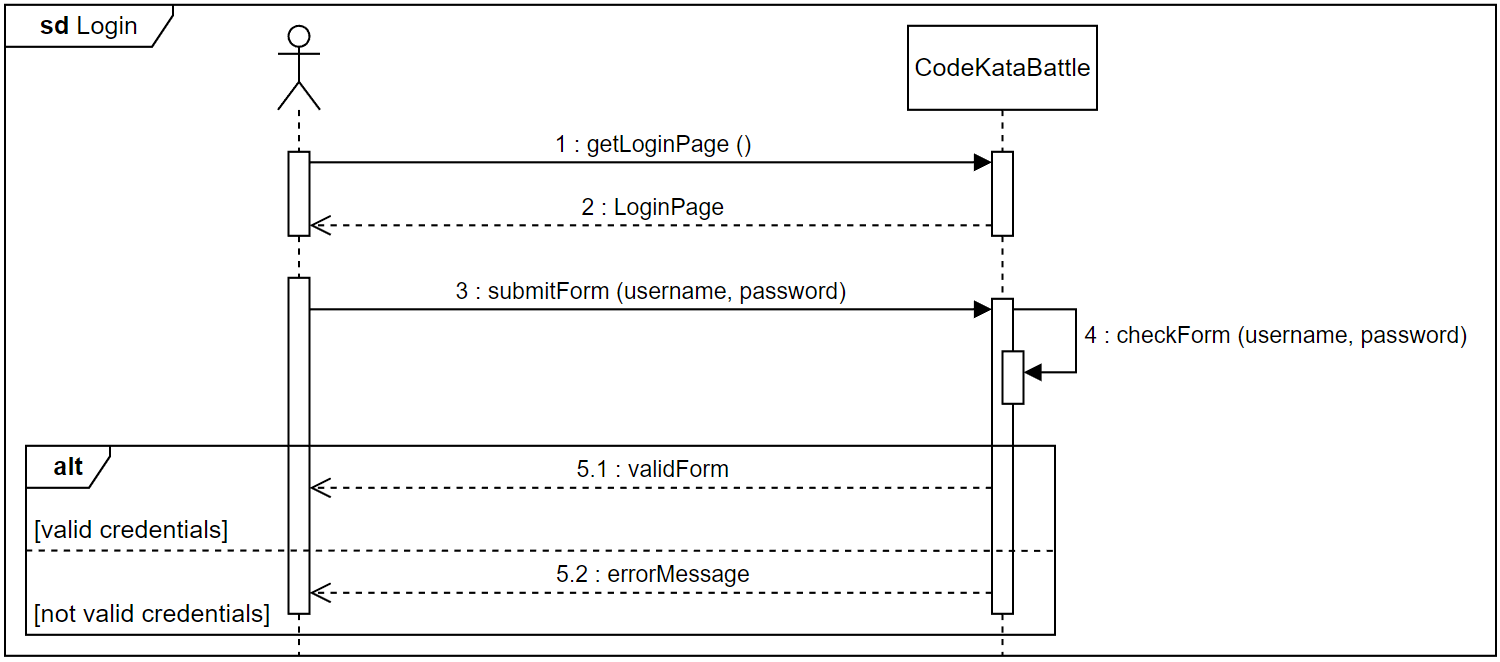
\includegraphics[width=0.9\linewidth]{images/login.png}\end{figure}}
        {\arabic{useCase}\stepcounter{useCase}}
        {Login}
        {Student, educator}
        {The actor clicks on the login button}
        {
        \begin{enumerate}
            \item The actor requires the login page by clicking the log-in button in the welcome page
            \item The system shows the login page to the actor
            \item The actor inserts credentials and send it to the system
            \item The system processes the information and shows a success message redirecting the user to the home page
        \end{enumerate}
        }
        {The actor is logged, and the homepage is displayed}
        {
        \begin{itemize}
            \item A wrong username or password is submitted
            \item A student tries to log in as educator and viceversa
        \end{itemize}
        }
        {In case of exception the system will notify user with a human-readable message}

        % usecase (Student, Educator) for checking the profile
        \usecase{%\begin{figure}[H]\centering\includegraphics[width=0.9\linewidth]{images/tournamentaccess.png}\end{figure}%
        }        
        {\arabic{useCase}\stepcounter{useCase}}
        {Checking the profile}
        {Educator}
        {The actor clicks on profile button}
        {
        \begin{enumerate}
            \item The actor clicks on profile button
            \item The system shows the profile page
            \item The actor can check his profile and eventually change personal information with edit button
        \end{enumerate}
        }
        {The actor is in the profile page}
        {
        \begin{itemize}
            \item The actor is not signed-in
        \end{itemize}
        }
        {In case of exception the system will notify user with a human-readable message}

        % usecase (Student) for visualizing all tournaments
        \usecase{%\begin{figure}[H]\centering\includegraphics[width=0.9\linewidth]{images/tournamentstud.png}\end{figure}%
        }        
        {\arabic{useCase}\stepcounter{useCase}}
        {Access to available tournaments}
        {Student}
        {The actor just logged in or clicked on the home button}
        {
        \begin{enumerate}
            \item The actor requires the home page
            \item The system shows the home page to the actor
            \item The actor can now check all the availabòe tournaments
        \end{enumerate}
        }
        {The actor is on the home page}
        {
        \begin{itemize}
            \item There are no active tournaments 
        \end{itemize}
        }
        {In case of exception the system will notify user with a human-readable message; the system cannot check if the right role is select during registration}

        % usecase (Student) for joining a specific tournament
        \usecase{%\begin{figure}[H]\centering\includegraphics[width=0.9\linewidth]{images/tournamentaccess.png}\end{figure}%
        }        
        {\arabic{useCase}\stepcounter{useCase}}
        {Join a specific tournament}
        {Student}
        {The actor clicks on the join tournament button}
        {
        \begin{enumerate}
            \item The actor enters the home page
            \item The system shows the home page to the actor
            \item The actor clicks on the join button of the desired tournament
            \item The system shows the enrolled page with the new tournament
        \end{enumerate}
        }
        {The actor is on the enrolled page}
        {
        \begin{itemize}
            \item The tournament selected by the actor is closed 
            \item The actor cannot join the selected tournament
        \end{itemize}
        }
        {In case of exception the system will notify user with a human-readable message}

        % usecase (Student, Educator) for the research of a tournament by the name
        \usecase{%\begin{figure}[H]\centering\includegraphics[width=0.9\linewidth]{images/tournamentaccess.png}\end{figure}%
        }        
        {\arabic{useCase}\stepcounter{useCase}}
        {Search a specific tournament}
        {Student, Educator}
        {The actor goes to tournament details page}
        {
        \begin{enumerate}
            \item The actor clicks the search tab on the left of any page
            \item The system shows the search page to the actor
            \item The actor fills thge form with the name of the searched tournament
            \item The system shows the matching tournaments
        \end{enumerate}
        }
        {The actor is in the search page}
        {
        \begin{itemize}
            \item The actor searches a wrong string (null or invalid characters)
            \item There are no matching active tournaments
        \end{itemize}
        }
        {In case of exception the system will notify user with a human-readable message}

        % usecase (Student) for joining a specific battle with the creation of a group
        \usecase{%\begin{figure}[H]\centering\includegraphics[width=0.9\linewidth]{images/tournamentaccess.png}\end{figure}%
        }        
        {\arabic{useCase}\stepcounter{useCase}}
        {Join a specific tournament}
        {Student}
        {The actor clicks on create and join battle button}
        {
        \begin{enumerate}
            \item The actor enters the tournament details page
            \item The system shows the tournament details page to the actor
            \item The actor clicks on the desired battle in the selected tournament
            \item The actor clicks on the create and join battle button or join on your own if it is alone
            \item The system shows the tournament details page with the new group
        \end{enumerate}
        }
        {The actor is in the tournament details page}
        {
        \begin{itemize}
            \item The selected battle is in a tournament where the actor is not enrolled
            \item The battle is already closed
            \item The educators that manages the battle does not accept the new group
        \end{itemize}
        }
        {In case of exception the system will notify user with a human-readable message}

        % usecase (Student) for joining a specific group in a battle
        \usecase{%\begin{figure}[H]\centering\includegraphics[width=0.9\linewidth]{images/tournamentaccess.png}\end{figure}%
        }        
        {\arabic{useCase}\stepcounter{useCase}}
        {Join a specific tournament}
        {Student}
        {The actor clicks the join button}
        {
        \begin{enumerate}
            \item The actor enters the tournament details page
            \item The system shows the tournament details page to the actor
            \item The actor clicks on the desired battle in the selected tournament
            \item The actor clicks on an already existing group
            \item The actor requires the access to the selected group by clicking on join
            \item The system shows the tournament details page with a message
        \end{enumerate}
        }
        {The actor is in the tournament details page}
        {
        \begin{itemize}
            \item The selected battle is in a tournament where the actor is not enrolled
            \item The battle is already closed
            \item The group does not accept the new student
            \item The group is already at maximum capacity
        \end{itemize}
        }
        {In case of exception the system will notify user with a human-readable message}

        % usecase (Student) for accessing the battle repository
        \usecase{%\begin{figure}[H]\centering\includegraphics[width=0.9\linewidth]{images/tournamentaccess.png}\end{figure}%
        }        
        {\arabic{useCase}\stepcounter{useCase}}
        {Join a specific tournament}
        {Student}
        {The actor goes to tournament details page}
        {
        \begin{enumerate}
            \item The actor enters the tournament details page
            \item The system shows the tournament details page to the actor
            \item The actor clicks on the repository button linked to the repository 
            \item The actor is redirected to the GitHub repository linked to the battle selected
        \end{enumerate}
        }
        {The actor is in the tournament details page and has another tab with the requestet repository}
        {
        \begin{itemize}
            \item The selected battle is in a tournament where the actor is not enrolled
            \item The battle is already closed
        \end{itemize}
        }
        {In case of exception the system will notify user with a human-readable message}

        % usecase (Student, Educator) for accessing all battle rankings
        \usecase{%\begin{figure}[H]\centering\includegraphics[width=0.9\linewidth]{images/tournamentaccess.png}\end{figure}%
        }        
        {\arabic{useCase}\stepcounter{useCase}}
        {Check the ranking of a specific battle}
        {Student, Educator}
        {The actor goes to tournament details page}
        {
        \begin{enumerate}
            \item The actor enters the tournament details page
            \item The system shows the tournament details page to the actor
            \item The actor clicks on a battle in the selected tournament 
            \item The actor can check the ranking in the details of the battle
        \end{enumerate}
        }
        {The actor is in the tournament details page}
        {
        \begin{itemize}
            \item There are no partecipants
        \end{itemize}   
        }
        {In case of exception the system will notify user with a human-readable message}

        % usecase (Student) for accessing all tournaments rankings
        \usecase{%\begin{figure}[H]\centering\includegraphics[width=0.9\linewidth]{images/tournamentaccess.png}\end{figure}%
        }        
        {\arabic{useCase}\stepcounter{useCase}}
        {Check the ranking of a specific tournament}
        {Student}
        {The actor clicks leaderboard button}
        {
        \begin{enumerate}
            \item The actor requires the enrolled page 
            \item The system shows the enrolled page
            \item The actor clicks on details of a tournament
            \item The system shows the details of the tournament 
            \item The actor clicks on leaderbord button
            \item The system shows the leaderboard page
            \item The actor can check the ranking of the selected tournament
        \end{enumerate}
        }
        {The actor is in the leaderbord page of the selected tournament}
        {
        \begin{itemize}
            \item There are no partecipants
        \end{itemize}
        }
        {In case of exception the system will notify user with a human-readable message}

        % usecase (Educator) for accessing all tournaments rankings
        \usecase{%\begin{figure}[H]\centering\includegraphics[width=0.9\linewidth]{images/tournamentaccess.png}\end{figure}%
        }        
        {\arabic{useCase}\stepcounter{useCase}}
        {Check the ranking of a specific tournament}
        {Educator}
        {The actor clicks leaderboard button}
        {
        \begin{enumerate}
            \item The actor search a tournament
            \item The system shows the corresponding tournament in the search page
            \item The actor clicks on detail on the desired tournament
            \item The system shows the details of the tournament 
            \item The actor clicks on leaderbord button
            \item The system shows the leaderboard page
            \item The actor can check the ranking of the selected tournament
        \end{enumerate}
        }
        {The actor is in the leaderbord page of the selected tournament}
        {
        \begin{itemize}
            \item There are no partecipants
        \end{itemize}
        }
        {In case of exception the system will notify user with a human-readable message}

        % usecase (Educator) for creating a new tournament
        \usecase{%\begin{figure}[H]\centering\includegraphics[width=0.9\linewidth]{images/tournamentaccess.png}\end{figure}%
        }        
        {\arabic{useCase}\stepcounter{useCase}}
        {Create a tournament}
        {Educator}
        {The actor clicks on create button on create tournament page}
        {
        \begin{enumerate}
            \item The actor enters the create tournament page
            \item The system shows the create tournament page to the actor
            \item The actor compile the form
            \item The actor clicks the create button to submit the form
            \item The system shows the manage tournament page to the actor with the new tournament
        \end{enumerate}
        }
        {The actor is in the manage tournament page}
        {
        \begin{itemize}
            \item The actor tries to create a tournament with invalid data
            \item The actor tries to create a tournament with invalid battles
            \item The actor tries to create a tournament with invalid collaborator invintations
        \end{itemize}
        }
        {In case of exception the system will notify user with a human-readable message}
        
        % usecase (Educator) for accessing all managed tournaments
        \usecase{%\begin{figure}[H]\centering\includegraphics[width=0.9\linewidth]{images/tournamentaccess.png}\end{figure}%
        }        
        {\arabic{useCase}\stepcounter{useCase}}
        {Manage a tournament}
        {Educator}
        {The actor goes to manage tournament page}
        {
        \begin{enumerate}
            \item The actor enters the manage tournament page
            \item The system shows the manage tournament page to the actor
            \item The actor selects the desired tournament
            \item The system shows the possible action for the selected tournament
        \end{enumerate}
        }
        {The actor is in the manage tournament page}
        {
        \begin{itemize}
            \item The actor tries to access an unmanaged tournament
            \item The actor tries to access a closed tournament
        \end{itemize}
        }
        {In case of exception the system will notify user with a human-readable message}

        % usecase (Educator) for creating a new battle
        \usecase{%\begin{figure}[H]\centering\includegraphics[width=0.9\linewidth]{images/tournamentaccess.png}\end{figure}%
        }        
        {\arabic{useCase}\stepcounter{useCase}}
        {Add a battle to a tournament}
        {Educator}
        {The actor clicks on add battle in the managed tournament page}
        {
        \begin{enumerate}
            \item The system shows the create battle page
            \item The actor compiles all the elements required by the form 
            \item The actor submits the form 
            \item The system show the managed tournament page with the modified tournament
        \end{enumerate}
        }
        {The actor is in the manage tournament page on the modified tournament with the new battle}
        {
        \begin{itemize}
            \item The form is not compiled correctly 
            \item The tournament selected is already closed 
        \end{itemize}
        }
        {In case of exception the system will notify user with a human-readable message}

        % usecase (Educator) for adding a new educator to a tournament
        \usecase{%\begin{figure}[H]\centering\includegraphics[width=0.9\linewidth]{images/tournamentaccess.png}\end{figure}%
        }        
        {\arabic{useCase}\stepcounter{useCase}}
        {Add a new educator to a tournament}
        {Educator}
        {The actor clicks on add collaborator in the managed tournament page}
        {
        \begin{enumerate}
            \item The system shows the managed tournament page with the possibility to add collaborators
            \item The actor insert the email in the corresponding form
            \item The actor clicks on invite
            \item The system show the managed tournament page with the modified tournament
        \end{enumerate}
        }
        {The actor is in the manage tournament page on the modified tournament with the pending invitation}
        {
        \begin{itemize}
            \item The email does not correpond to another educator 
            \item The tournament selected is already closed 
        \end{itemize}
        }
        {In case of exception the system will notify user with a human-readable message}

        % usecase (Educator) for closing a tournament 
        \usecase{%\begin{figure}[H]\centering\includegraphics[width=0.9\linewidth]{images/tournamentaccess.png}\end{figure}%
        }        
        {\arabic{useCase}\stepcounter{useCase}}
        {Close a tournament}
        {Educator}
        {The actor clicks on close button on a specific tournament in manage tournament page}
        {
        \begin{enumerate}
            \item The actor enters the manage tournament page
            \item The system shows the manage tournament page
            \item The actor select the desired tournament 
            \item The actor clicks on close button in the selected tournament
            \item The system shows the manage tournament page and the tournament is closed
        \end{enumerate}
        }
        {The actor is in the manage tournament page on the modified tournament with the closed tournament}
        {
        \begin{itemize}
            \item The tournament is already closed
        \end{itemize}
        }
        {In case of exception the system will notify user with a human-readable message}

        % usecase (Educator) for evaluating a battle manually
        \usecase{%\begin{figure}[H]\centering\includegraphics[width=0.9\linewidth]{images/tournamentaccess.png}\end{figure}%
        }        
        {\arabic{useCase}\stepcounter{useCase}}
        {Evaluate a battle}
        {Educator}
        {The actor enters the manage battle page}
        {
        \begin{enumerate}
            \item The actor enters the manage battle page
            \item The system shows the manage battle page
            \item The actor clicks on selected battle
            \item The actor fill the form with the manual evaluation grades
            \item The actor clicks publish button
            \item The system shows the manage battle page and the manual evaluation is complete
        \end{enumerate}
        }
        {The actor is in the manage battle page}
        {
        \begin{itemize}
            \item The battle is not yet closed
            \item The form is not compiled correctly
        \end{itemize}
        }
        {In case of exception the system will notify user with a human-readable message}



















    \section{Performance requirements}
        The performance requirements needed to ensure the reliability and the availability of the system are: 
        \begin{itemize}
            \item The backend must be scalable based on the number of active user, reactive. 
                It must be able to magae a proper load-balancing to ensure performance also when numeorus users are conneccted togehter to the platform. 
            \item The frontend must be modeled to be user-friendly, so that also educators and students that does not work often with technology can use the platform. 
                The interface must also be fluid and handle asynchronous interaction to ensure a certain level of usability even when the connection is not too stable. 
            \item The system must have a security level that ensure availability and protect the system and users' data from malicious pepole. 
            \item Since the notifications are used to alert the unser mainly on deadlines, they must be delivered in a short time (in the order of some minutes). 
            \item The system must also adapt when the number of user increase suddently (e.g., when the final rankings are published multiple users login into a single tournament page). 
        \end{itemize}

    \section{Design constraints}
        \subsection{Standards compliance}
        The specifications described in this document must be followed during all the development process and the final product must adhere to these. \\
        The source code of the system must be commented to ensure that all the specifications are met. \\
        The data used by the application must be treated accordingly to the GDPR. 

        \subsection{Hardware limitations}
        The application requires a device that can be a mobile one or a personal computer. \\
        In both cases the device needs an internet connection to retrieve data from the server. 

        \section{Software system attributes}
        \subsection{Reliability}
        To ensure enhanced reliability performance, conduct all scheduled system maintenance during nighttime. 
        Additionally, be aware that certain system functionalities depend on external APIs; however, a failure in one of them should not result in a complete system failure. 
        Prioritize the prevention of data loss by employing redundant storage methods.

        \subsection{Availability}
        The system must deliver its functionalities with an availability of 99.5\% or higher, meaning it should be inaccessible for less than two days each year.
        To meet this objective, ensure high redundancy for the most crucial components of the system.

        \subsection{Security}
        To safeguard sensitive user data, the system should gather only essential information, storing it in an encrypted database. 
        The connection between the application must adhere to contemporary standard protocols like HTTPS.
        We must encrypt email and passwords. 
        The latter one also needs salt. 

        \subsection{Maintainability}
        Source code and related documentation should have comprehensive comments and be consistently updated. 
        Emphasize modularity, low coupling, and high cohesion between components during the design and development phases. 
        Specifically, ensure that the modularity of the frontend and backend allows developers to update the backend seamlessly without users experiencing any disruptions.

        \subsection{Portability}
        The application should be accessible on prominent mobile operating systems, targeting at least the latest releases. 
        The web application must be compatible with the most recent browsers. 
        Optimal efficiency can be achieved by judiciously reusing a significant portion of the codebase across both mobile and web platforms through the use of cross-platform tools.


\chapter{Formal analysis with Alloy}















\chapter{Effort spent}
    The table below offers a concise overview of the hours invested by each group member, along with a brief description of their contributions. 
    Dates where the same amount of time was dedicated by all members usually indicates collaborative efforts.
    \begin{table}[H]
        \centering
        \begin{tabular}{cccc}
            \textbf{Date}   & \textbf{Rossi}            & \textbf{Sharoubim}            & \textbf{Description}                          \\ \hline
            22-10-2023      & 1                         & 0                             & Repository setup and file structure           \\ 
            28-10-2023      & 3                         & 1                             & First chapter initial content                 \\ 
            29-11-2023      & 4                         & 4                             & Part of second and third chapters             \\
            30-11-2023      & 2                         & 2                             & Initial class diagram                         \\
            05-12-2023      & 0                         & 6                             & Graphical user interfaces                     \\
            05-12-2023      & 2                         & 2                             & Graphical user interfaces                     \\
            06-12-2023      & 3                         & 3                             & Class diagrams                                 \\
            09-12-2023      & 1                         & 1                             & Use case diagrams                             \\
            10-12-2023      & 2                         & 2                             & Use case diagrams                                              \\
            xx-xx-xxxx      & -                         & -                             &                                               \\
            xx-xx-xxxx      & -                         & -                             &                                               \\
            xx-xx-xxxx      & -                         & -                             &                                               \\
            xx-xx-xxxx      & -                         & -                             &                                               \\ \hline
            \textbf{Total}  & 16                        & 19                            & -                                             \\  
        \end{tabular}
    \end{table}


\chapter{References}

    \textbf{Diagrams} - https://app.diagrams.net
    \\
    \textbf{UI Mockup} - https://webflow.com



\end{document}